%% Copernicus Publications Manuscript Preparation Template for LaTeX Submissions
%% ---------------------------------
%% This template should be used for copernicus.cls
%% The class file and some style files are bundled in the Copernicus Latex Package, which can be downloaded from the different journal webpages.
%% For further assistance please contact Copernicus Publications at: production@copernicus.org
%% https://publications.copernicus.org/for_authors/manuscript_preparation.html


%% Please use the following documentclass and journal abbreviations for discussion papers and final revised papers.

%% 2-column papers and discussion papers
\documentclass[gmd, manuscript]{copernicus}



%% Journal abbreviations (please use the same for discussion papers and final revised papers)


% Advances in Geosciences (adgeo)
% Advances in Radio Science (ars)
% Advances in Science and Research (asr)
% Advances in Statistical Climatology, Meteorology and Oceanography (ascmo)
% Annales Geophysicae (angeo)
% Archives Animal Breeding (aab)
% ASTRA Proceedings (ap)
% Atmospheric Chemistry and Physics (acp)
% Atmospheric Measurement Techniques (amt)
% Biogeosciences (bg)
% Climate of the Past (cp)
% DEUQUA Special Publications (deuquasp)
% Drinking Water Engineering and Science (dwes)
% Earth Surface Dynamics (esurf)
% Earth System Dynamics (esd)
% Earth System Science Data (essd)
% E&G Quaternary Science Journal (egqsj)
% Fossil Record (fr)
% Geographica Helvetica (gh)
% Geoscientific Instrumentation, Methods and Data Systems (gi)
% Geoscientific Model Development (gmd)
% History of Geo- and Space Sciences (hgss)
% Hydrology and Earth System Sciences (hess)
% Journal of Micropalaeontology (jm)
% Journal of Sensors and Sensor Systems (jsss)
% Mechanical Sciences (ms)
% Natural Hazards and Earth System Sciences (nhess)
% Nonlinear Processes in Geophysics (npg)
% Ocean Science (os)
% Primate Biology (pb)
% Proceedings of the International Association of Hydrological Sciences (piahs)
% Scientific Drilling (sd)
% SOIL (soil)
% Solid Earth (se)
% The Cryosphere (tc)
% Web Ecology (we)
% Wind Energy Science (wes)


%% \usepackage commands included in the copernicus.cls:
%\usepackage[german, english]{babel}
%\usepackage{tabularx}
%\usepackage{cancel}
%\usepackage{multirow}
%\usepackage{supertabular}
%\usepackage{algorithmic}
%\usepackage{algorithm}
%\usepackage{amsthm}
%\usepackage{float}
%\usepackage{subfig}
%\usepackage{rotating}
\graphicspath{{final_figures/}}

\begin{document}

\title{Update and evaluation of the ozone dry deposition in the Oslo~CTM3 v1.0}


% \Author[affil]{given_name}{surname}

\Author[1]{Stefanie}{Falk}
\Author[2,a]{Amund}{S{\o}vde Haslerud}
%\Author[]{}{}

\affil[1]{Department of Geosciences, University of Oslo, Oslo, Norway}
\affil[2]{CICERO Center for International Climate Research, Oslo, Norway}
\affil[a]{Kjeller Vindteknikk, Kjeller, Norway}

%% The [] brackets identify the author with the corresponding affiliation. 1, 2, 3, etc. should be inserted.



\runningtitle{Update of ozone dry deposition in the Oslo~CTM3}

\runningauthor{Falk}

\correspondence{Stefanie Falk (stefanie.falk@geo.uio.no)}



\received{}
\pubdiscuss{} %% only important for two-stage journals
\revised{}
\accepted{}
\published{}

%% These dates will be inserted by Copernicus Publications during the typesetting process.


\firstpage{1}

\maketitle



\begin{abstract}
 High concentrations of ozone in ambient air are hazardous not only to humans but to the ecosystem in general. The impact of ozone damage on vegetation and agricultural plants in combination with advancing climate change may affect food security in the future. While the future scenarios in themselves are uncertain, there are limiting factors constraining the accuracy of surface ozone modeling also at present: The distribution and amount of ozone precursors and ozone depleting substances, the stratosphere-troposphere exchange as well as scavenging processes. Removal of any substance through gravitational settling or by uptake by plants and soil is referred to as dry deposition. The process of dry deposition is important for predicting surface ozone concentrations and understanding the observed amount and increase of tropospheric background ozone. The conceptual dry deposition velocities are calculated following a resistance-analogous approach wherein aerodynamic, quasi laminar, and canopy resistances are key components, but these are hard to measure explicitly. We present an update of the dry deposition scheme implemented in the Oslo~CTM3. We change from a purely empirical dry deposition parameterization to a more process-based one which is taking the state of the atmosphere and vegetation into account. We examine the sensitivity of the scheme to various parameters, e.g. the stomatal conductance-based description of the canopy resistance and the choice of ozone surface resistance, and evaluate the resulting modeled ozone dry deposition with respect to observations and multi-model studies. Individual dry deposition velocities are now available for each land surface type and agree generally well with observations. We also estimate the impact on the modeled ozone concentrations at the surface. We show that the global annual total ozone dry deposition decreases with respect to the previous model version ($-37\,\unit{\%}$), leading to an increase in surface ozone of more than $100\,\unit{\%}$ in some regions. While high sensitivity to changes in dry deposition to vegetation is found in the tropics and the northern hemisphere, the largest impact on global scales is associated with the choice of prescribed ozone surface resistance over the ocean and deserts.
\end{abstract}

%\copyrightstatement{TEXT}
\introduction  %% \introduction[modified heading if necessary]
\label{sec:intro}
Ozone is an important trace gas for all lifeforms on Earth. Depending on the place of its occurrence it has either a positive or negative connotation. In the stratosphere, ozone absorbs most of the ultraviolet (UV)-light from the sun within the range of 100--315\,\unit{nm}, thus shielding the Earth's surface from the most harmful UV-radiation. In addition, ozone is a potent greenhouse gas in both, stratosphere and troposphere. With a radiative forcing of $0.40 \pm 0.20\,\unit{W\,m^{-2}}$, it is placed third, only surpassed by \chem{CO_2} and \chem{CH_4} \citep[Chapter 8]{IPCC2013}.\\
In the troposphere and in particular in ambient air, ozone is considered as a highly toxic pollutant. Since the industrial revolution, tropospheric background ozone concentrations have been increasing in the northern hemisphere \citep[Chapter 2]{IPCC2013}. In recent years, the number of episodes of peak concentrations has been, in general, decreasing in North America and Europe due to the implementation of air quality regulations \citep[e.g.,][]{ESA:Fleming2018, ESA:Mills2018}. At the same time, fast developing countries, like e.g., China or India, saw a significant increase in ozone related air pollution. Continuously high concentrations of ambient air ozone are hazardous to the whole ecosystem. It is estimated that ozone is cause to an increase in pre-mature deaths \citep{WHO2008}, an average global loss of yield in the four major crops (wheat, rice, maize, and soybean) of about $3-15\,\unit{\%}$ \citep{PJ:Ainsworth2017} as well as $7\,\unit{\%}$ loss in primary production in forestry \citep{GCB:Wittig2009,EP:Matyssek2012}. The impact of ozone damage on vegetation and agricultural plants may affect food security in the future especially in Asia \citep{GCB:Tang2013,NCC:Tai2014,AE:Chuwah2015,GCB:Mills2018} and might be an important additional feedback to climate change \citep{Nat:Sitch2007}.\\
Elevated ozone levels at a site may originate from both, the local production of ozone from its precursors, which are transported, and from advection of ozone itself. Long-range ozone transport occurs regularly and might be most important in regions that otherwise lack precursors. Tropospheric ozone is produced in complex photochemical cycles involving precursor gases such as carbon monoxide (\chem{CO}) or volatile organic substances (VOCs -- also known as hydrocarbons) in the presents of nitrogen oxides (\chem{NO_x}). A typical reaction mechanism for \chem{CO} is sketched in the following. In a sequence of rapid reactions a peroxyl radical \chem{HO_2^\bullet} is formed through an initial reaction of \chem{CO} with a hydroxyl radical \chem{^\bullet OH}.
Via a reaction between \chem{HO_2^\bullet} and \chem{NO}, \chem{NO_2} is formed which is then photolyzed. The resulting atomic oxygen reacts then with \chem{O_2} (and also under the presence of available co-reactants) to form an ozone molecule.
Such a cycle leads to a net production via:
\begin{reaction}
  \chem{CO} + 2\chem{O_2} + h\nu \rightarrow \chem{CO_2} + \chem{O_3}.
\end{reaction}
Similar cycles involving VOCs exist \citep{ACP:Monks2015}. Another source of tropospheric ozone is downward transport from the stratosphere via stratosphere-troposphere exchange (STE) \citep{WMO2014}. Based on observations, STE might only amount to $10\,\unit{\%}$ ($550 \pm 140\,\unit{Tg\,a^{-1}}$) of the total global ozone budget in the troposphere, while ozone from chemical production is estimated to be $5000\,\unit{Tg\,a^{-1}}$ \citep{ACP:Monks2015}. Ozone is removed from the atmosphere by photochemical reactions or scavenging processes. Major sinks are photolysis followed by a reaction with water vapor to from \chem{OH},
reactions with \chem{HO_2}, titration reactions, and dry deposition. We will come back to the latter later in this section and cover the implemented scheme in more detail in Section~\ref{subsec:DryDep}.

Since ozone is highly reactive, its global mean life-time in the troposphere is roughly $22$ days but ranges between a few days in the tropical boundary layer to up to $1$ year in the upper troposphere \citep{JGR:Stevenson2005,ACP:Young2013}. The abundance of tropospheric ozone therefore varies, e.g., with time of the day, season, altitude, location \citep{ACP:Schnell2015}, or weather conditions in general \citep{ACP:Otero2018}. Typical concentrations of surface ozone range from $10\,\unit{ppb}$ over the tropical Pacific to $100\,\unit{ppb}$ in the downwind areas of highly emitting sources \citep[Chapter 8]{IPCC2013}. This variability poses a challenge on both, trend analysis from observations as well as validation and intercomparison of models. From the observational side, the number of long-term observations (started before the 1950s) is limited and restricted to mainly European sites. Most of these indicate a doubling of tropospheric ozone since the 1950s \citep[Chapter 2]{IPCC2013}. But especially the very low pre-industrial ozone abundance cannot be reproduced by the likes of most models. These early observations, however, were subject to interference by other species, e.g., \chem{SO_2}. Among the participating models in the Atmospheric Chemistry and Climate Model Intercomparison Project (ACCMIP), there is a general tendency to underestimate tropospheric ozone burden (e.g., $10-20\,\unit{\%}$ negative bias at $250\,\unit{hPa}$ in the southern hemisphere (SH) tropical region) \citep[Chapter 8]{IPCC2013}. With respect to surface ozone, \citet{ACP:Schnell2015} conclude that all ACCMIP models, which reported hourly surface ozone, tend to overestimate surface ozone values in North America and Europe in comparison with available observations. A key to fathom these slightly contradicting results may lie in the used dry deposition schemes.\\
Removal of any substance from the atmosphere which is not involving rain, e.g., through gravitational settling or by uptake by plants, soil, and water, is referred to as dry deposition. The process of dry deposition is important for predicting surface ozone concentrations and understanding the observed amount and increase of tropospheric background ozone. It is estimated that $1000 \pm 200\,\unit{Tg\,a^{-1}}$ of ozone are removed from the atmosphere by dry deposition processes \citep{ACP:Monks2015}. A newer study by \citet{ACP:Luhar2018}, however, indicates much lower amounts ($722.8 \pm 87.3\,\unit{Tg\,a^{-1}}$) due to lower dry deposition to the oceans. Conceptually, dry deposition is a product between near-surface ozone concentration \chem{[O_3](z_0)} (e.g. the lowermost model level) and a dry deposition velocity $v^\chem{O_3}_\text{DD}$. Species dependent dry deposition velocities $v^i_\text{DD}$, which are synonymously referred to as conductance $G^i$, for any gaseous species $i$, are typically calculated following a resistance-analogous approach
\begin{equation}
  v^i_\text{DD} = \frac{1}{R_a + R^i_b + R^i_c},
  \label{eq:drydep_velo}
\end{equation}
wherein aerodynamic $R_a$, quasi-laminar layer $R^i_b$, and canopy resistances $R^i_c$ are key components \citep{AE:Wesely1989,ACP:Seinfeld2006}. For all gases, $R_a$ is the same, while $R^i_b$ and $R^i_c$ vary from gas to gas and also depend on land surface types (e.g., ice/snow, water, urban, desert, agricultural land, deciduous forest, coniferous forest etc.). Originally, \citet{AE:Wesely1989} used fixed seasonal average dry deposition resistances for each land surface type. For all three types of resistances in this Wesely-type parameterization, more process-oriented formulations have been developed and validated over the years. \citet{ACP:Luhar2017} have validated ozone dry deposition to the ocean with respect to three different formulations of surface resistances.
Based on the global atmospheric composition reanalysis performed in the ECWMF project Monitoring Atmospheric Composition and Climate (MACC) \citep{MACC-II} and a more realistic process-based oceanic deposition scheme, \citet{ACP:Luhar2018} found that the ozone dry deposition to oceans amounts to $98.4 \pm 30.0\,\unit{Tg\,a^{-1}}$. In particular, \citet{ACP:Luhar2018} found that the average surface resistance of ozone over ocean ($r_c=2200\,\unit{sm^{-1}}$) is highly overestimated in most models.
An update on the ozone surface resistance over snow and ice covered surfaces has been provided from combined model and observation studies \citep[][$v^\chem{O_3}_\text{ice/snow} = 1/10000\,\unit{m\,s^{-1}}$]{ACP:Helmig2007}. Canopy conductance is parameterized at the single-leaf-level (stomatal conductance) for various plant function types (PFT) as well as for single plant species based on empirical studies \citep{PTRS:Jarvis1976, BallBerry1987, ACP:Simpson2012, ICP:MappingManual2017}. But progress has also been made on process-oriented modeling of stomatal conductance \citep{AFM:Anderson2000,PP:Buckley2017}. The variety of differing formulations and choices of parameters leads to a wide spread of results in model intercomparisons \citep{ACP:Hardacre2015,AE:Derwent2018} and about $20\,\unit{\%}$ uncertainty on the resulting total dry deposition \citep{ACP:Monks2015}.\\

In Section~\ref{sec:model_des}, we will briefly describe the Oslo~CTM3, give a detailed account of the new dry deposition scheme (Section~\ref{subsec:DryDep}) as well as present pre-processing of meteorological input data to compute necessary input to the dry deposition scheme such as the begin and duration of the greening season (GDAY, GLEN) and photosynthetic photon flux density (PPFD) (Section~\ref{subsec:pre-pro}). In Section~\ref{sec:eval}, we present sensitivity tests with respect to a manifold of parameters in the dry deposition scheme (Section~\ref{subsec:sens}) and validate our results with respect to results from the multi-model intercomparison of \citet{ACP:Hardacre2015} (Section~\ref{subsec:model}), the MACC-reanalysis (Section~\ref{subsec:macc}), and to surface ozone observations (Section~\ref{subsec:obs}). In Section~\ref{sec:conc}, we will summarize and discuss our results and draw conclusions for further development of the model.
%%%%%%%%%%%%%%%%%%%%%%%%%%%%
%%%%%%%%%%%%%%%%%%%%%%%%%%%%
\section{Model description}
\label{sec:model_des}
The Oslo~CTM3 is an offline, three dimensional, global chemistry transport model (CTM). The key components of the Oslo~CTM3 have been described and evaluated by \citet{GMD:Sovde2012}. A detailed account of the capabilities of the Oslo~CTM3 in simulating anthropogenic aerosol forcing in the past and recent past using the Community Emission Data System (CEDS) historical emission inventory \citep{GMD:Hoesly2018} is given by \citet{GMD:Lund2018}. The Oslo~CTM3 can also be coupled to the Model of Emissions of Gases and Aerosols from Nature (MEGAN v2.10) \citep{ACP:Guenther2006}. A publication focussing on this is planned.

%Although the ozone depleting events in the polar boundary layer (Section~\ref{sec:intro}) are important to understand surface ozone abundance in Arctic regions in spring-time, no parameterization of these processes is implemented in the Oslo~CTM3 as of now.\\
While the meteorological data driving the Oslo~CTM3 is given at a resolution of T159N80L60, with the highest model level at $0.02\,\unit{hPa}$, it is very time and memory consuming to run the Oslo~CTM3 with full chemistry at this resolution. Therefore, we reduced the horizontal resolution to $2.25^\circ\times2.25^\circ$ in our experiments. In the following, we will give a detailed account of the new dry deposition scheme and the equations that we use.
%%%%%%%%%%%%%%%%%%%%%%%%%%%%
\subsection{Ozone dry deposition scheme}
\label{subsec:DryDep}
In the original dry deposition scheme, the state of the atmosphere was not taken into account. Dry deposition velocities were rather parameterized following the work of \citet{AE:Wesely1989} with parameter updates from \citet{JGR:Hough1991}. This means that seasonal day and night average deposition velocities for different land surface types (water, forest, grass, tundra/desert, and ice and snow) were in use. Day was distinguished from night by solar zenith angles below $90\,\unit{^\circ}$. Winter was defined by temperatures below $273.15\,\unit{K}$ for gridboxes containing land masses. For ocean, winter and summer parameters are equal in this parameterization, therefore no distinctive treatment was needed for ocean gridboxes. In addition, a reduced uptake due to snow cover above $1\,\unit{m}$ for forest and $10\,\unit{cm}$ for grass/tundra, respectively, was taken into account. We will refer to this parameterization as \emph{Wesely scheme}.\\

Regarding the new dry deposition scheme, we mainly follow \citet{ACP:Simpson2012} in their description of dry deposition used in the European Monitoring and Evaluation Programme (EMEP) MSC-W model \citep[see also,][]{Emberson2000, WASP:Simpson2003, AE:Tuovinen2004}, which is used for air quality modeling implementing the Convention on Long-Range Transboundary Air Pollution (CLRTAP). We will refer to the new scheme as \emph{mOSaic scheme} throughout the rest of the paper. The mOSaic scheme is a more physical approach compared to the previously used Wesely scheme, because it takes state (e.g., pressure, temperature)  of the atmosphere as well as dynamics (e.g., wind stress) of the boundary layer into account. To a certain degree, the global variety of plants and their variability throughout the seasons is also acknowledged. The mOSaic scheme is implemented for the gaseous species \chem{O_3}, \chem{H_2O_2}, \chem{NO_2}, \chem{PAN}, \chem{SO_2}, \chem{NH_3}, \chem{HCHO}, and \chem{CH_3CHO}. Since \chem{CO} has a very small uptake and is not included in \citet{WASP:Simpson2003,ACP:Simpson2012}, the Wesely parameterization is kept. In addition to the gaseous species, \citet{ACP:Simpson2012} also modify aerosol deposition velocities, namely black carbon (BC) and organic carbon (OC), sulfuric aerosols (\chem{SO_4}, \chem{MSA}) and secondary organic aerosols (SOA), but we have not updated our model with respect to these.

As displayed in Eq.~(\ref{eq:drydep_velo}), the dry deposition computation is subdivided into contributions from three different resistances. The main idea of a mosaic approach is to calculate these resistances separately for each land surface type $k$ in each grid cell: $R_a^k$,$R^{i,k}_b$, and $R^{i,k}_c$.
The grid cell average dry deposition velocity $\overline{v}_\mathrm{DD}^{i}$ is then defined by weighting each individual $v_\mathrm{DD}^{i,k}$ by the corresponding land fraction factor $f_k$:
\begin{equation}
  \overline{v}_\mathrm{DD}^{i} = \sum_k{f_k v_\mathrm{DD}^{i,k}}
  \label{eq:ddep_velo_wa}
\end{equation}

\subsubsection{Aerodynamic resistance}
\label{subsubsec:Ra}
In general, the aerodynamic resistance describes the turbulent transport of any substance down to the surface. To derive $R_a^k$, we follow \citet{WASP:Simpson2003,ACP:Simpson2012} and compute a local friction velocity at reference height $z_\mathrm{ref}$ \citep[Eq.~(52),][]{ACP:Simpson2012}
\begin{equation}
  u_*^k = \frac{\overline{u}(z_\mathrm{ref})\cdot\kappa}{\ln{(\frac{z_\mathrm{ref}-d_k}{z_0^k})}-\Psi_m(\frac{z_\mathrm{ref}-d_k}{L})+\Psi_m(\frac{z_0^k}{L})},
  \label{eq:local_fric_vel}
\end{equation}
with the average wind speed $\overline{u}(z_\mathrm{ref})$ at reference height, the K\'{a}rm\'{a}n constant $\kappa = 0.40$, the integrated stability equation for momentum $\Psi_m$ \citep[e.g.,][]{Garratt1992}, a grid average Obukhov length $L$, deplacement height $d_k$, and roughness length $z_0^k$ ($d_k=0.78\cdot h_k(\mathrm{lat})$, $z_0^k=0.07\cdot h_k(\mathrm{lat})$ for forests, $d_k=0.7\cdot h_k(\mathrm{lat})$, $z_0^k=0.1\cdot h_k(\mathrm{lat})$ for vegetation other than forests). Taking the height of vegetation in to consideration, we have chosen the model level such that $\overline{z}_\mathrm{ref}\approx 45\,\unit{m}$. Using the derived $u_*^k$ from Eq.~(\ref{eq:local_fric_vel}), a local Obukhov length $L_k$ can be obtained from \citep[Eq.~(8),][]{ACP:Simpson2012}:
\begin{equation}
  L_k = - \frac{\rho c_p T_\mathrm{2m} u_*^k}{\kappa g H}.
\end{equation}
Herein, $H$ is the sensible heat flux, $g$ is the standard gravitational acceleration, $c_p$ the specific heat capacity, and $T_{2m}$ the $2\,\unit{m}$ temperature. With these, we can compute the aerodynamical resistance for each land surface type \citep[Eq.~(8.8),][]{WASP:Simpson2003}
\begin{equation}
  R_a^k = \frac{1}{\kappa u_*^k}\left[{\ln{\left(\frac{z_\mathrm{ref}-d_k}{z_0^k}\right)}-\Psi_h\left(\frac{z_\mathrm{ref}-d_k}{L_k}\right)+\Psi_h\left(\frac{z_0^k}{L_k}\right)}\right],
\end{equation}
with the integrated stability equation for heat $\Psi_h$ \citep[e.g.,][]{Garratt1992}. Both integrated stability functions ($\Psi_m$, $\Psi_h$) and corresponding parameters are listed in supplement~S.1.
%%%%%%%%%%%%%%%%%%%%%%%%%%%%
\subsubsection{Quasi-laminar layer resistance}
\label{subsubsec:Rb}
The quasi-laminar layer resistance $R_b^{i,k}$ is species specific and differs over land and ocean surfaces.
%%%%%%%%%%%%%%%%%%%%%%%%%%%%
Over land, we use \citep[Eq.~(53),][]{ACP:Simpson2012}
\begin{equation}
  R_b^{i,k} = \frac{2}{\kappa u_*} \cdot \left(\frac{\text{Sc}_i}{\text{Pr}}\right)^{\frac{2}{3}},
  \label{eq:Rb}
\end{equation}
wherein $\text{Pr}$ is the Prandtl number (0.72 for air and other gases) and $\text{Sc}_i$ is the Schmidt number for a gas $i$. Eq.~(\ref{eq:Rb}) differs from a similar formulation in \citet{ACP:Seinfeld2006} by a factor of roughly $1.25$. From $\text{Sc}_i = \nu/D_i$, with the kinematic viscosity of air $\nu$, we derive a Schmidt number in water equivalent:
\begin{equation}
  \text{Sc}_i = \frac{D_\chem{H_2O}}{D_i} \cdot \text{Sc}_\chem{H_2O},
\end{equation}
with the molecular diffusivity for any gas $D_i$, the Schmidt number of water ($\text{Sc}_\chem{H_2O}=0.6$) and its molecular diffusivity ($D_\chem{H_2O}=0.21\cdot10^{-4}\,\unit{m^2\,s^{-1}}$). The used ratios $D_\chem{H_2O}/D_i$ are taken from \citet[][Table S18]{ACP:Simpson2012}.\\

%%%%%%%%%%%%%%%%%%%%%%%%%%%%
Over ocean, we use \citep[Eq.~(54),][]{ACP:Simpson2012}
\begin{equation}
  R_b^i = \frac{1}{\kappa u_*}\cdot\ln\left({\frac{z_0}{D_i}\cdot \kappa u_*}\right)
\end{equation}
with an imposed lower threshold of $10\,\unit{s\,m^{-1}}$ and an upper limit of $1000\,\unit{s\,m^{-1}}$. The computation of roughness length $z_0$ over ocean is divided into a \emph{calm} and a \emph{rough} sea case, with a threshold of $3\,\unit{m\,s^{-1}}$. For calm sea, we apply the following upper limit \citep[][with a slightly higher coefficient of $0.135$]{Hinze1975,Garratt1992}
\begin{equation}
  z_0^\text{calm} = \text{min}\left\{2\cdot10^{-3}, 0.135 \cdot \frac{\nu}{u_*}\right\}.
\end{equation}
The kinematic viscosity of air $\nu$ herein can be computed from 
\begin{equation}
  \nu = \frac{\mu}{\rho} = \frac{\mu(T)}{\frac{P_0}{T\cdot R_\text{air}}}.
  \label{eq:kinematic_viscosity}
\end{equation}
For the temperature dependent dynamic viscosity of air $\mu(T)$, we chose a linear fit to Sutherland's law through the origin within the temperature range $\{T \in \mathbb{R} | (243.15 < T < 313.15)\,\unit{K}\}$: $\mu(T) = 6.2\cdot 10^{-8}\,\unit{kg\,m^{-1}\,s^{-1}\,K^{-1}} \cdot T$. But despite its rough accuracy, we found that the choice of $\mu(T)$ has no effect on $\overline{R}_b^{i,k}$ (Supplement~S.2: Figs.~S1--S2). In Eq.~(\ref{eq:kinematic_viscosity}), $\rho$ is substituted by the air density using the ideal gas law. $P_0$ is the surface pressure, as $T$ the $2\,\unit{m}$ temperature is chosen, and $R_\text{air}$ is the universal gas constant for air.
The rough sea case follows the method of \citet{QJRMS:Charnock1955,JPO:Wu1980}:
\begin{equation}
  z_0^\text{rough} = \text{min}\left\{2\cdot10^{-3}, 0.018 \cdot \frac{u^2_*}{g}\right\}
\end{equation}
with a gravitational acceleration $g = 9.836\,\unit{m\,s^{-2}}$. The allowed maximum roughness length in both cases is set to $2\,\unit{mm}$. Since the $z_0$ computed with this parameterization are rather small ($0 < z_0^\text{calm} < 1\cdot 10^{-4}\,\unit{m}$, $0 < z_0^\text{rough} < 2 \cdot 10^{-3}\,\unit{m}$), $R^i_b$ is set to its lower limit of $10\,\unit{s\,m^{-1}}$ in about $91\,\unit{\%}$ of all cases (see Supplement~S.2: Fig.~S3). 
%%%%%%%%%%%%%%%%%%%%%%%%%%%%
\subsubsection{Surface resistance}
\label{subsubsec:Rc}
The surface resistance consists of both stomatal and non-stomatal resistances.\\ 
%%%%%%%%%%%%%%%%%%%%%%%%%%%%
%\subsubsection*{Stomatal conductance}
The stomatal conductance is a measure of the rate of \chem{CO_2} exchange and evapotranspiration through the stomata of a leaf. There are several environmental conditions affecting the opening and closing of the stomata and hence the capability of respiration (e.g., light, available water, etc.). Stomata sluggishness, a state in which the stomata can no longer fully close, has been reported as ozone induced damage \citep{SR:Hoshika2015}, but is not taken into account in our formulation. To reflect part of the underlying mechanism, the leaf-level molar stomatal conductance in the mOSaic scheme is computed using a common multiplicative ansatz \citep{BallBerry1987, ICP:MappingManual2017}:
%
\begin{equation}
  g^k_\text{sto, m} = g^k_\text{max, m} \cdot f^k_\text{phen} \cdot f^k_\text{light} \cdot \max{\left\{f^k_\text{min}, f^k_T \cdot f^k_D \cdot f^k_\text{SW}\right\}}.
  \label{eq:stomatal}
\end{equation}
%
The factors herein are normalized and vary within the range $0-1$. They account for leaf phenology ($f_\text{phen}$), light ($f_\text{light}$), temperature ($f_T$), water vapor pressure deficit ($f_D$), and soil water content ($f_\text{SW}$). All factors differ with land use type $k$. For clarity reasons, we drop this index in the following, as long as it is not necessary for the equation's completeness. The maximum molar stomatal conductance is given by $g^k_\text{max, m}$ which is in units of \unit{mmol\,s^{-1}\,m^{-2}}. A unit conversion to \unit{m\,s^{-1}} is necessary in our model:

\begin{equation}
  g^k_{\text{sto}} = g_{\text{sto, m}}^k \cdot R \cdot \frac{T_0}{P_0}.
\end{equation}
Herein, $R$ is the universal gas constant. To annotate the differing units, we use the index $\text{m}$ in Eq.~(\ref{eq:stomatal}).\\

The temperature adjustment $f_T$ is computed from
%
\begin{equation}
  f_T = \frac{T_\text{2m}-T_\text{min}}{T_\text{opt}-T_\text{min}} \cdot \left(\frac{T_{\text{max}}-T_\text{2m}}{T_{\text{max}}-T_\text{opt}}\right)^\beta, 
\end{equation}
with $\beta = \frac{T_\text{max}-T_\text{opt}}{T_\text{opt}-T_\text{min}}$. The parameters $T_\text{min}$, $T_\text{max}$ and $T_\text{opt}$ are tabulated for various plant functional types. All parameters are taken from \citet[][Tables S16, S19]{ACP:Simpson2012}. Since $f_T$ turns negative outside the range defined by $T_\text{min}$, $T_\text{max}$, we impose a lower limit of $0.01$ for numerical reasons.

The water vapor deficit (VPD) is proportional to the saturation partial pressure of water ($P_\chem{H_2O}^s$) and relative humidity ($\text{RH}$)
%
\begin{equation}
  \text{VPD} = P_\chem{H_2O}^s \cdot (1 - \text{RH}/100).
\end{equation}
%
Using tabulated values of $f_\text{min}$, $D_\text{min}$, $D_\text{max}$, the water vapor pressure deficit penalty factor $f_D$ can be computed:
%
\begin{equation}
  f_D = f_\text{min}+(1-f_\text{min}) \cdot \frac{D_\text{min} - \text{VPD}}{D_\text{min}-D_\text{max}}.
\end{equation}

The penalty factor with respect to available soil water ($\text{SW}$) $f_\text{SW}$ is defined as 
%
\begin{equation}
  f_\text{SW} =
  \begin{cases}
    1 & \quad \emph{if} \quad \text{SW} \geq 0.5,\\
    2 \cdot \text{SW}  & \quad \emph{if} \quad \text{SW} < 0.5.
  \end{cases}
\end{equation}
SW is evaluated at a soil depths of $0.28-1\,\unit{m}$, which corresponds to SWVL3 in OpenIFS.

The phenology of a plant typically describes its life-cycle throughout a year, e.g., at mid latitudes and for deciduous species, it starts with the emergence of leafs in spring and ends in fall. In the mOSaic scheme, phenology is parameterized with respect to the start of the greening season (SGS) and its end (EGS). Details about our treatment of these are given in Section~\ref{subsubsec:greening}. In summary, our adaption of the $f_\text{phen}$ parameterization reads as follows:
%
\begin{equation}
  f_\text{phen} =
  \begin{cases}
    \emph{if} \quad \text{GLEN $\ge$ 365} & \quad 1 \quad \emph{(explicitly excluding tropics)} \\
    \emph{if} \quad \text{GDAY = 0}  & \quad 0 \\
    \emph{else}  & \quad 
    \begin{cases}
      \emph{if} \quad \text{GDAY} \le \phi_\text{AS}  & \quad \phi_a \\
      \emph{if} \quad \text{GDAY} \le \phi_\text{AS} + \phi_e  & \quad \phi_b+(\phi_c-\phi_b)\cdot(\text{GDAY}-\phi_\text{AS})/\phi_e\\
      \emph{if} \quad \text{GDAY} \le \text{GLEN} - \phi_\text{AE} - \phi_f  & \quad \phi_c\\
      \emph{if} \quad \text{GDAY} \le \text{GLEN} - \phi_\text{AE}  & \quad \phi_d+(\phi_c-\phi_d)\cdot(\text{GLEN}-\phi_\text{AE}-\text{GDAY})/\phi_f\\
      \emph{else} & \quad \phi_d
    \end{cases}
  \end{cases}
  \label{eq:fphen}
\end{equation}
%
Herein, we use the SGS and EGS derived parameters day of greening season (GDAY), the time elapsed starting at the SGS, and the total length of the greening season (GLEN), the time span between EGS and SGS. The parameters $\phi_a$, $\phi_b$, $\phi_c$, and $\phi_d$ define start or end points in the five phases of phenology in the mOSaic scheme, while $\phi_e$, $\phi_f$, $\phi_\text{AS}$, and $\phi_\text{AE}$ control the temporal timing (Fig.~\ref{fig:phenology}). If GLEN is zero we are, e.g., in Arctic regions and there is no vegetation anyway, therefore $f_\text{phen}=0$. Before the start of the greening season ($\text{GDAY}=0$) $f_\text{phen}=0$. Since this phenology is tuned to northern hemisphere (NH) mid latitudes, it does not apply to the tropics. We therefore decided to set $f_\text{phen}=1$ if GLEN is greater or equal to 365 which is the case in the tropics.
%
\begin{figure}[t]
  \includegraphics[width=8.3cm]{fig01}
  \caption{Sketch of the five different phases in plant phenology $f_\text{phen}$ in accordance to Eq.~(\ref{eq:fphen}).}
  \label{fig:phenology}
\end{figure}

Light in the wavelength band $400-700\,\unit{nm}$ to which the plant chlorophyll is sensitive is called photosynthetic active radiation (PAR). The integral of PAR over these wavelengths is the photosynthetic photon flux density (PPFD). The correction factor $f_\mathrm{light}$ in response to varying PPFD is:
\begin{equation}
  f_\text{light} = 1-\text{exp}(-\alpha_\text{light}\cdot \text{PPFD}).
  \label{eq:flight}
\end{equation}


%%%%%%%%%%%%%%%%%%%%%%%%%%%%
%\subsubsection*{Non-stomatal conductance}
In the mOSaic scheme, non-stomatal conductances are explicitly calculated for \chem{O_3}, \chem{SO_2}, \chem{HNO_3}, and \chem{NH_3}. For all other species, an interpolation between \chem{O_3} and \chem{SO_2} values is carried out.
The non-stomatal conductance for \chem{O_3} consists of two terms, one depending on vegetation type and one depending on the soil/surface. For each land surface type $k$, we can write
\begin{equation}
  G_\text{ns}^{\chem{O_3}, k} = \frac{\text{SAI}_k}{r_\text{ext}} + \frac{1}{R_\text{inc}^k + R_\text{gs}^{\chem{O_3},k}}.
  \label{eq:non-stomata-cond}
\end{equation}
$\text{SAI}_k$ is the surface area index for vegetation type $k$, which is $\text{LAI}$ plus a value that represents cuticles and other surfaces. The external leaf resistance is defined by
\begin{equation}
  r_\text{ext} = 2000\,\unit{s\,m^{-1}}\cdot F_T.
\end{equation}
Herein $F_T$ is a temperature correction factor for temperatures below $-1\,\unit{^\circ C}$ and $\{F_T \in \mathbb{R} | (1 \leq F_T \leq 2)\}$
\begin{equation}
  F_T = \exp{(-0.2\cdot(1+\theta_\text{2m}))}.
\end{equation}
$\theta_\text{2m}$ is the $2\,\unit{m}$ temperature in \unit{^\circ C}. For most land surface types, $\text{SAI} \equiv \text{LAI}$. Some exceptions are: 
%
\begin{equation}
  \text{SAI} = 
  \begin{cases}
    \text{LAI}+1 & \emph{if} \quad \text{\emph{forest / wetland}},\\
    \text{LAI}\cdot 5/3.5 & \emph{if} \quad \text{\emph{cropland}, 1st part of growing season},\\
    \text{LAI} + 1.5 & \emph{if} \quad \text{\emph{cropland}, 2nd part of growing season},\\
    0 & \emph{if} \quad \text{\emph{cropland}, winter}.
  \end{cases}
  \label{eq:SAI}
\end{equation}
%
Extending the mOSaic scheme to the southern hemisphere, we use the growing season for crops defined in Table~\ref{tab:growing_season}.
%
\begin{table}[t]
  \caption{Definition of growing season for crops used in the Oslo~CTM3 in northern hemisphere (NH) and southern hemisphere (SH).}
  \begin{tabular}{lrr}
    \tophline
    & 1st part & 2nd part \\
    & (days) & (days) \\
    \middlehline
    NH & 90--140 & 141--270 \\
    SH & 272--322 & 323--452 \\
    \bottomhline
  \end{tabular}
  %\belowtable{} % Table Footnotes
  \label{tab:growing_season}
\end{table}
%

In this way, vegetation affects the conductance also by being there, not only by uptake through the stomata. The in-canopy resistance $R_\text{inc}$ \citep{AE:Erisman1994} is then modified with respect to each (vegetated) land surface type in $k$
\begin{equation}
  R_\text{inc} = b \cdot \text{SAI}_k \cdot \frac{h_k(\text{lat})}{u_*},
\end{equation}
where $h_k(\text{lat})$ is the latitude dependent vegetation height (see explanation at the end of this section) and $b = 14\,\unit{m^{-1}}$ is an empirical constant. The canopy resistance described in \citet{ACP:Simpson2012} does not take temperature and snow into account and is zero for non-vegetated surfaces, but we will adopt the correction previously used in the Oslo~CTM3 Wesely scheme.\\
As initially mentioned, the necessary depth of snow to cover a certain type of vegetation differs. Therefore, we calculate a snow cover fraction $f_\text{snow}$ using the snow depth $S_D$, which is available in units of meter of water equivalent from the meteorological input data, scaled to $10\,\unit{\%}$ of the vegetation height.
$R_\text{gs}^{\chem{O_3},k}$ is tabulated. We correct for temperature by $F_T$ and for snow cover fraction:
\begin{equation}
  \frac{1}{R_\text{gs}^{\chem{O_3},k}} = \frac{1-f_\text{snow}^k}{\hat{R}_\text{gs}^{\chem{O_3},k}} + \frac{f_\text{snow}^k}{R_\text{snow}^{\chem{O_3},k}}.
\end{equation}

The bulk canopy conductance is then defined as:
\begin{equation}
  G_c^k = \text{LAI} \cdot g^k_\text{sto, m} + G^k_\text{ns}, 
\end{equation}
wherein $\text{LAI}$ is the one-sided leaf area index taken from ISLSCP2 FASIR, $g_\text{sto}$ the leaf-level stomatal conductance, and $G_\text{ns}$ the bulk non-stomatal conductance.\\

%%%%%%%%%%%%%%%%%%%%%%%%%%%%%%%%%%%%%%%%%%%%%%%%%%%%
\subsubsection{Latitude dependent vegetation height}
The vegetation height $h_k(\text{lat})$ as described by \citet{ACP:Simpson2012} is linearly decreasing with latitude between $60\,\unit{^\circ}$ and $74\,\unit{^\circ N}$. To adapt this to a global model, we made a few additional assumptions. The tabulated height for each vegetation type $h_k$ in the mOSaic scheme is regarded as constant at mid latitudes ($40\,\unit{^\circ}-60\,\unit{^\circ}$). Towards the poles, we decrease the height of each vegetation type using the same rate as described in \citet{ACP:Simpson2012}. At a latitude of $74\,\unit{^\circ}$ a minimum height of $3/10 \cdot h_k$ is reached and kept constant. Towards the equator, we increase the height linearly so that at a latitude of $10\,\unit{^\circ}$ a maximum height of $2 \cdot h_k$ is reached which is then held constant. We also assume symmetry in both hemispheres. Presuming a typical tree height of $20\,\unit{m}$ at mid latitudes, this step-wise function yields a height of $8\,\unit{m}$ at high latitudes and $40\,\unit{m}$ in the tropics which is not unrealistic. For four example PFTs, results are shown in the Supplement (S.3, Fig.~S4).

\subsubsection{Mapping of land surface types}
The Oslo~CTM3 is configured to read land surface types from, either \href{https://daac.ornl.gov/cgi-bin/dataset_lister.pl?p=29}{ISLSCP2} product from MODIS or Community Land Model (\href{http://www.cgd.ucar.edu/tss/clm/}{CLM})~2 categories, which have to be mapped to the land surface types used in the mOSaic scheme (Fig.~\ref{fig:pft_mapping}). For both, MODIS and CLM~2 land surface categories, snow and ice cover is estimated from input meteorology, while $f_L^\text{water}$ is defined as $1-\sum_{k} f_L^k$. From the MODIS category \emph{Barren or sparsely vegetated}, everything polward from $60\,\unit{^\circ}$ is defined as tundra, while everything equatorward is categorized as desert. This mapping differs from the one used in the Wesely scheme.

\begin{figure*}[t]
  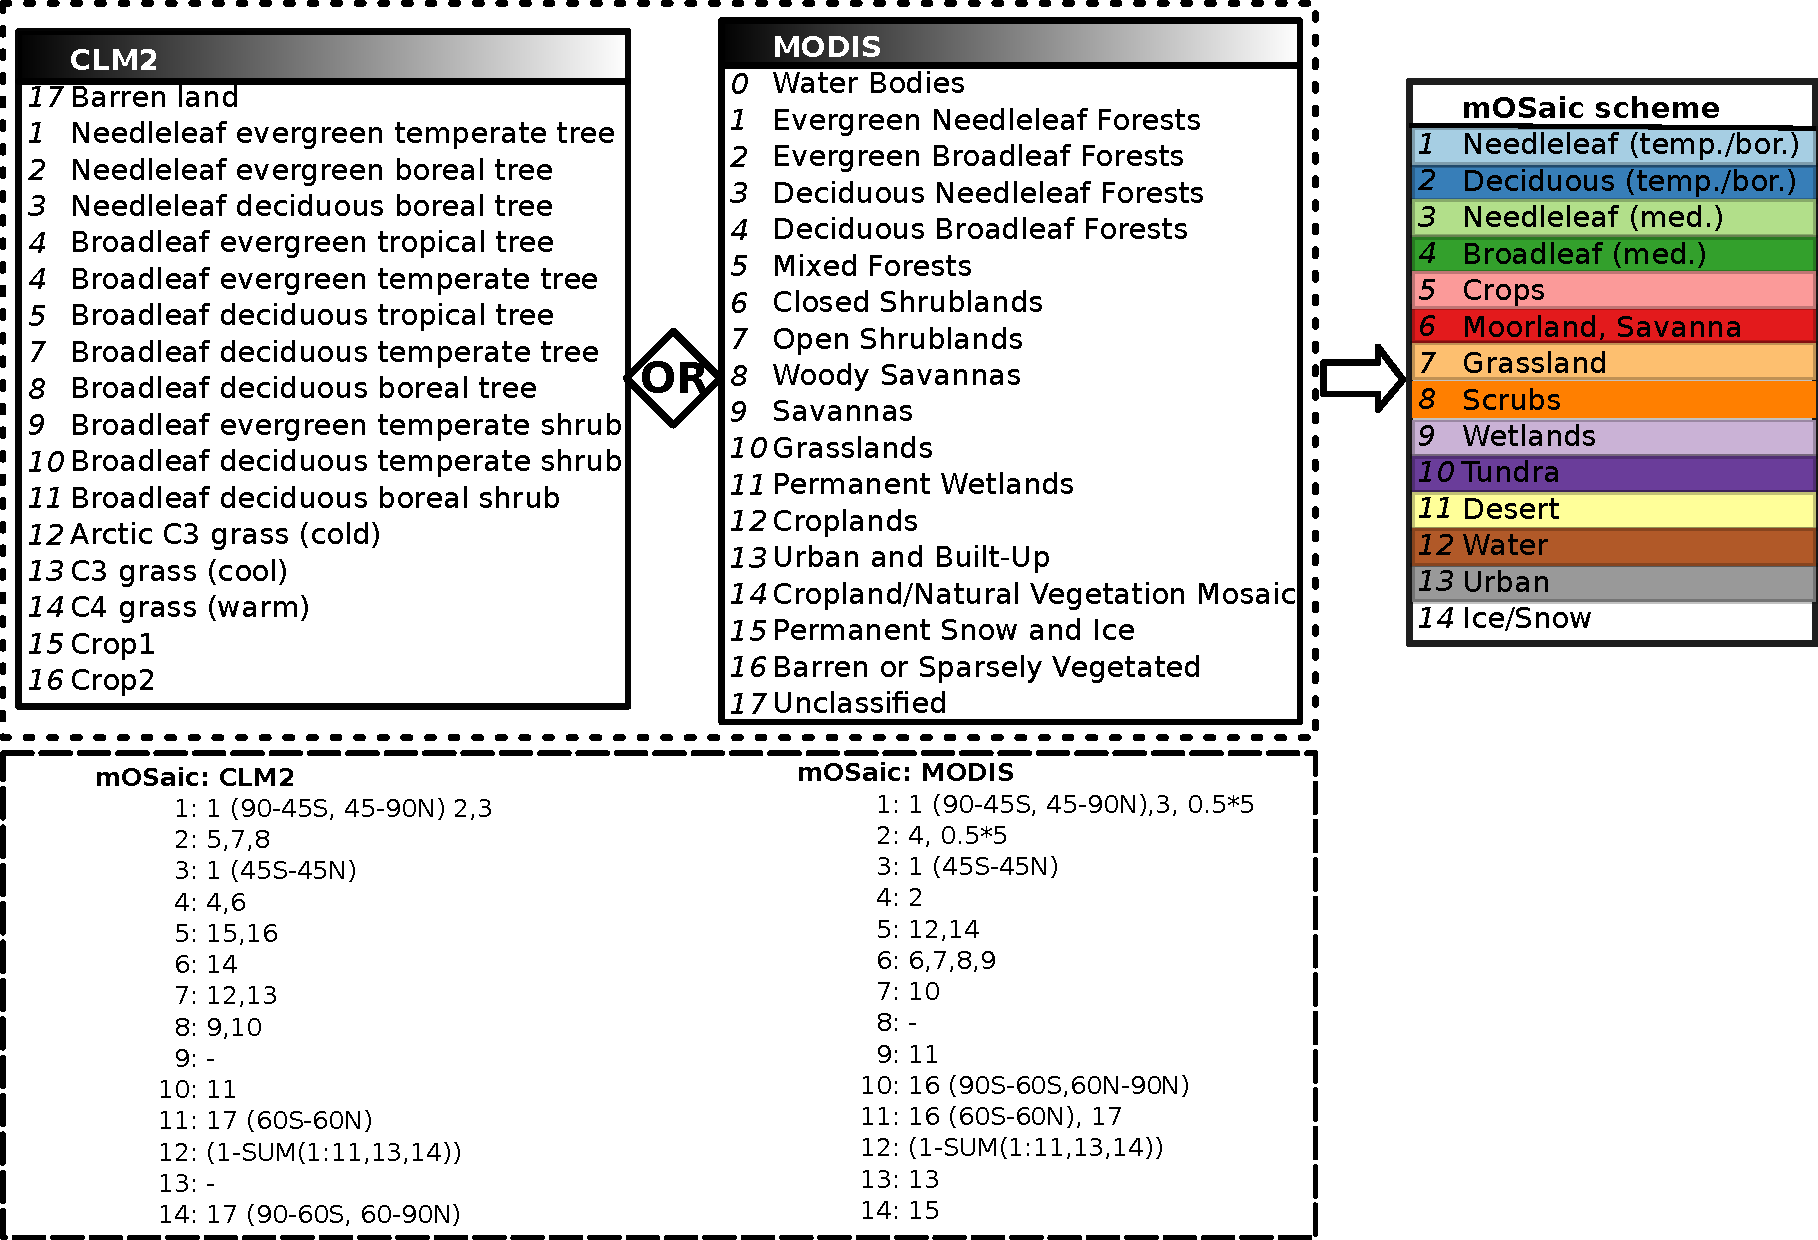
\includegraphics[width=12cm]{fig02}
  \caption{Mapping of land surface categories. Either land surface categories from ISLSCP2 product of MODIS or the Community Land Model (CLM)~2 can be chosen for mapping to the land surface types we use in the mOSaic scheme. Water bodies of MODIS are actually not mapped. For both, MODIS and CLM~2 land surface categories, snow and ice cover is estimated from input meteorology, while water is defined as $1-\sum_{k} f_L^k$. From MODIS category \emph{Barren or sparsely vegetated}, everything polward from $60\,\unit{^\circ}$ is defined as tundra, while everything equatorward is categorized as desert.}
  \label{fig:pft_mapping}
\end{figure*}
%
%%%%%%%%%%%%%%%%%%%%%%%%%%%%
\subsection{Pre-processing}
\label{subsec:pre-pro}
As mentioned in the previous section, there are two variables needed for computing the stomatal conductance which are not directly available from the meteorological input data. The greening season, as the time of the year in the mid and high latitudes when it is most likely for plants to grow, and the photosynthetic photon flux density, as the amount of light that plants need to photosynthesize. In the following, we present the necessary pre-processing of the variables. It is planned to implement an online computation of these variables into the Oslo~CTM3 later on.
%%%%%%%%%%%%%%%%%%%%%%%%%%%%
\subsubsection{Greening season}
\label{subsubsec:greening}
In Eqs.~(\ref{eq:non-stomata-cond}--\ref{eq:SAI}), \citet{ACP:Simpson2012} use prescribed start of growing season (SGS) and end of growing season (EGS) at $50\,\unit{^\circ N}$ ($d_\text{SGS}$, $d_\text{EGS}$) together with lapse rates ($\nabla d_\text{SGS}$, and $\nabla d_\text{EGS}$) to define phenology and dry deposition over agricultural areas. For the growing season of crops in the computation of non-stomatal conductances, we use also prescribed values (Table~\ref{tab:growing_season}), while for the stomatal conductances, as shown in Eq.~(\ref{eq:fphen}), we use the SGS and EGS derived parameters: day of greening season (GDAY), the time elapsed starting at the SGS, and the total length of the greening season (GLEN), the time span between EGS and SGS. Since the parameterization of SGS and EGS in \citet{ACP:Simpson2012} is not applicable in a global model, another latitude dependent parameterization is needed. First, we used a parameterization which was already implemented in the Oslo~CTM3 and which had been adopted from the Sparse Matrix Operational Kernel Emissions -- Biogenic Emission Inventory System (SMOKE-BEIS; \href{https://www.epa.gov/air-emissions-modeling/biogenic-emission-inventory-system-beis}{https://www.epa.gov/air-emissions-modeling/biogenic-emission-inventory-system-beis}). SMOKE-BEIS has fixed values for SGS and EGS for all regions but NH mid latitudes ($23\,\unit{^\circ} < \text{lat} < 65\,\unit{^\circ}$), where it uses lapse rates of $\nabla d_\text{SGS} = 4.5$ and $\nabla d_\text{EGS} = 3.3$. As this parameterization is optimized for North America, it does not work well in Europe, e.g., most of northern Scandinavia has no allocated vegetation period. This basically results in a suppression of canopy resistance in northern Scandinavia.\\ 

In agriculture, there are different empirical rules to estimate the SGS and EGS. The simplest assumption is that greening starts after $5$ consecutive days with a daily average temperature above $5\,\unit{^\circ C}$ and vice versa for EGS. Other estimates use growing degree days \citep{JC:Levis2004,PO:Fu2014}, include soil moisture \citep{GCB:Fu2014}, or rely on satellite observations. A comprehensive evaluation of different techniques is given by \citet{GCB:Anav2017}. Another solution would be the usage of a proper land surface model, e.g. LPJ-GUESS, CLM, but the integration of such into the Oslo~CTM3 is not planned at the moment.

Based on the empirical rule ($5\,\unit{^\circ C}$-days), we have pre-processed our meteorological input data offline. We added some additional criteria to prevent for \emph{false spring}: If, within these $5$ days, the average temperature drops below or rises above $5\,\unit{^\circ C}$, the counter is reset, respectively. First, we used the $5\,\unit{^\circ C}$-days criteria for $45\,\unit{^\circ} < \text{lat} < 85\,\unit{^\circ}$ in the NH, but extended it also to $35\,\unit{^\circ} < \text{lat} < 65\,\unit{^\circ}$ in the SH. In all other cases and where the $5\,\unit{^\circ C}$-days criteria fails, we still use the SMOKE-BEIS parameterization. The described algorithm written in python~2.7 has been included as Supplement~S.4. An example map of the computed GLEN using the $5\,\unit{^\circ C}$-days criteria in both hemispheres is shown in Fig.~\ref{fig:glen_2015_she}.
%
\begin{figure}[t]
  \includegraphics[width=8.3cm, clip, trim={0.cm 1.75cm 0.cm 1.75cm}]{fig03}
  \caption{Pre-processing of greening season from meteorological surface temperature fields. Shown is the total length of the greening season (GLEN) for the year 2005. The $5\,\unit{^\circ C}$-days criteria has been used in both hemispheres mid--high latitudes. Ocean has been shaded to indicate that greening season will only affect land.}
  \label{fig:glen_2015_she}
\end{figure}
%
%%%%%%%%%%%%%%%%%%%%%%%%%%%%
\subsubsection{Photosynthetic photon flux density}
From OpenIFS an accumulated surface PAR is available. It is integrated both, spectrally (presumably $400-700\,\unit{nm}$) and temporally. For practical use in Eq.~(\ref{eq:flight}), we de-accumulate this field with respect to time and refer to the result as PPFD.

The main obstacle is that PAR has been accumulated since model start, so that the first field kept from the original OpenIFS simulation ($00\,\unit{UTC}$) is $12$ hours after model start ($12\,\unit{UTC}$ on the previous day). In other words, the first time step of each day in the Oslo~CTM3 has already accumulated PAR from $12\,\unit{UTC}$ on the previous day.
De-accumulation of times $03\,\unit{UTC}$ to $21\,\unit{UTC}$, simply means computing the difference
\begin{equation}
  \text{PPFD}(t_i) = \text{PAR}(t_{i+1})-\text{PAR}(t_i).
\end{equation}
For de-accumulation of the remaining time step, the best choice is subtracting the difference between $21\,\unit{UTC}$ and $12\,\unit{UTC}$ of the previous day
%
\begin{equation}
  \text{PPFD}(t=00\,\unit{UTC}) = \text{PAR}(t=00\,\unit{UTC}) - \left[\text{PAR}(t=21\,\unit{UTC}-1\,\unit{day})-\text{PAR}(t=12\,\unit{UTC}-1\,\unit{day})\right]
\end{equation}
%
and limit the result to positive values only. An example PAR de-accumulation for January 2nd 2005 is shown in Supplement~S.5 (Figs.~S5--S7).
The resulting PPFD fields are still accumulated over a time period of $3$ hours and should be divided by $3$. A \href{https://confluence.ecmwf.int/display/CKB/ERA-Interim\%3A+surface+photosynthetically+active+radiation+\%28surface+PAR\%29+values+are+too+low}{known issue} in the OpenIFS (cycles $\le$ c41r2) causes surface PAR values to be about $30\,\unit{\%}$ below observations. To counter this, we decided to refrain from the division at this stage, but need to bear this in mind for later OpenIFS cycles.

%%%%%%%%%%%%%%%%%%%%%%%%%%%%      
\section{Evaluation}
\label{sec:eval}
In this section, we present results from a manifold of Oslo~CTM3 model integrations testing different parameters of the mOSaic scheme. We focus on changes in ozone total dry deposition $\sum\chem{O_3^\text{DD}}$, dry deposition velocities $v^\chem{O_3}_\text{DD}$, concentrations in the lowermost model level $[\chem{O_3}](p_0)$, and tropospheric burden $\sum_\text{trop}\chem{O_3}$. We evaluate our results with respect to the multi-model comparison of ozone dry deposition by \citet{ACP:Hardacre2015} (Section~\ref{subsec:model}), the MACC-reanalysis (Section~\ref{subsec:macc}), and observations (Section~\ref{subsec:obs}). The Oslo~CTM3 is driven by meteorological input fields from \href{https://www.ecmwf.int/en/forecasts/documentation-and-support/evolution-ifs/cycle-38r1-summary-changes}{ECMWF -- OpenIFS cy38r1}. CEDS historical emission inventory \citep{GMD:Hoesly2018} is used for anthropogenic emissions, while biomass burning is covered in daily resolution by NASA's Global Fire Emissions Database, Version4 (GFEDv4). Biogenic emissions are taken from MEGAN-MACC output \citep{ACP:Sindelarova2014}, while emissions from soil and wetlands are computed by MEGAN. Resultant $\mathrm{NO_x}$ emissions are up-scaled to match Global Emissions InitiAtive (GEIA) inventory and are estimated to amount to $6.55\,\unit{Tg(N)\,a^{-1}}$. For oceanic emissions of \chem{CO}, we use predefined global fields from POET \citep{POET}. Emissions of \chem{CH_4} are taken from the EU project (EU GOCE 037048) Hydrogen, Methane and Nitrous oxide: Trend variability, budgets and interactions with the biosphere (HYMN) for the year 2003 and scaled to oceanic amounts of $\mathrm{CH_4}$ from NASA. In the following (Section~\ref{subsec:sens}), we will present the various model sensitivity studies.
%%%%%%%%%%%%%%%%%%%%%%%%%%%%
\subsection{Sensitivity studies}
\label{subsec:sens}
Due to significant differences between the mOSaic scheme and the previous Wesely scheme with respect to implementation, it is not possible to fully disentangle and trace back every single difference in results to a respective change. Therefore, we conducted one reference simulation denoted as \emph{mOSaic} and in total seven sensitivity studies to probe the parameter space for stomatal conductance (\emph{mOSaic\_offLight}, \emph{mOSaic\_offPhen}, and \emph{mOSaic\_SWVL1}), ozone surface resistance $R^\chem{O_3}$ (\emph{mOSaic\_ice}, \emph{mOSaic\_desert}, and \emph{mOSaic\_hough}), and emissions (\emph{mOSaic\_emis2014}). A reference simulation featuring the Oslo~CTM3 Wesely scheme has been conducted and will be referred to as \emph{Wesely\_type}, indicating that other implementations of the original work by \citet{AE:Wesely1989} may exist in other models.
All model experiments discussed in the following are summarized in Table~\ref{tab:simsum}. An \emph{x} therein denotes that the model was run exactly in the configuration and with parameters as has been described in Section~\ref{sec:model_des}.
For all model integrations, the meteorological reference year is 2005. This choice affects the direct comparison with data and studies that either show results based on decadal averages or differing years, because non-linearities in ozone formation and destruction make ozone concentrations sensitive to both, differences in local concentration of precursors and meteorological conditions \citep{JGR:Jin2013}.

First, we have a closer look at the influence of certain parameters on the stomatal conductance. As indicated by the names, \emph{mOSaic\_offLight} and \emph{mOSaic\_offPhen} are rather extreme scenarios completely switching off the sensitivity to light and phenology in Eq.~(\ref{eq:stomatal}) by setting $f_\text{light}$ and $f_\text{phen}$ to a fixed value of 1, respectively. Because of the underlying research project's focus on Arctic and alpine ecosystems, where water might only be available from upper soil layers, an experiment was conducted using the uppermost soil water level (SWVL1) in the implementation of $f_\text{SW}$. 
After this, we want to confirm the importance of choice of $R^\chem{O_3}$ for different land surface types. We conducted three experiments looking at a $R^\chem{O_3}_\text{ice/snow}$ update \citep{ACP:Helmig2007} (\emph{mOSaic\_ice}), observed $R^\chem{O_3}_\text{desert}$ \citep{AE:Gusten1995} (\emph{mOSaic\_desert}), and an approximation of $R^\chem{O_3}$ originally used in \emph{Wesely\_type} \citep{AE:Wesely1989, JGR:Hough1991}.
Finally, we run a simulation with emissions for the year 2014 instead of 2005 (\emph{EMEP\_emis2014}) to characterize the general influence of differing emissions on ozone.  

\begin{table*}[t]
  \caption{Summary of specifications of all simulations discussed in this section. For simplicity, only the tested parameters are listed. An x denotes that the model was run exactly in the configuration as has been described in Section~\ref{sec:model_des}.}
  \begin{tabular}{lccccccccc}
    \tophline
    \multirow{2}{*}{Simulation} & \multicolumn{3}{c}{mOSaic scheme} & \multicolumn{2}{c}{Greening season} & $R^\chem{O_3}$ & Emissions\\
    & $f_\text{phen}$ & $f_\text{light}$ & $f_\text{SW}$ & SMOKE-BEIS & $5\,\unit{^\circ C}$-days & & (year)\\
    \middlehline
    Wesely\_type      &  \multicolumn{3}{c}{n/a}   & x & n/a& \citet{AE:Wesely1989, JGR:Hough1991}  & 2005 \\
    mOSaic            &   x & x & x                &   &  x & \citet{ACP:Simpson2012}  & 2005 \\
    mOSaic\_offLight  &   x & 1 & x                &   &  x & \citet{ACP:Simpson2012}  & 2005 \\
    mOSaic\_offPhen   &   1 & x & x                &   &  x & \citet{ACP:Simpson2012}  & 2005 \\
    mOSaic\_SWVL1     &   x & x & VL1              &   &  x & \citet{ACP:Simpson2012}  & 2005 \\
    mOSaic\_ice       &   x & x & x                &   &  x & \citet{ACP:Simpson2012}; \citet{ACP:Helmig2007}$^\dagger$ & 2005 \\
    mOSaic\_desert    &   x & x & x                &   &  x & \citet{ACP:Simpson2012}; \citet{AE:Gusten1995}$^*$  & 2005 \\
    mOSaic\_emis2014  &   x & x & x                &   &  x & \citet{ACP:Simpson2012}  & 2014 \\
    mOSaic\_hough     &   x & x & x                &   &  x & \citet{AE:Wesely1989, JGR:Hough1991}$^\star$  & 2005 \\
    \bottomhline
  \end{tabular}
  \label{tab:simsum}
  \belowtable{$^\dagger\,R^\chem{O_3}_\text{ice/snow}=10000\,\unit{s\,m^{-1}}$; $^*\,R^\chem{O_3}_\text{desert}=800\,\unit{s\,m^{-1}}$; $^\star\,$For adapted values see Supplement~S.6} % Table Footnotes
\end{table*}
%
\begin{figure}[t]
  \includegraphics[width=8.3cm]{fig04}
  \caption{Relative difference between reference simulations \emph{mOSaic} and the \emph{Wesely\_type} with respect to (a) average surface ozone; (b) average ozone dry deposition velocity; (c) total amount of ozone removed from the atmosphere by dry deposition.}
  \label{fig:diff_maps}
\end{figure}
%
In Fig.~\ref{fig:diff_maps}, we show global distributions of the relative difference between \emph{mOSaic} and \emph{Wesely\_type} for surface ozone, dry deposition velocity, and total ozone dry deposition. The surface ozone increases globally except for some regions covered by tropical forest. Especially in desert regions in Africa, America, and Asia, the surface ozone increases by more than $100\,\unit{\%}$. Consistently, dry deposition velocities decrease globally by the same order of magnitude in these regions, while they increase over tropical forest. With respect to total dry deposition, the picture is a bit less clear. We find a decrease of total dry deposition of ozone in desert regions and ocean covered areas and an increase in regions covered by tropical forest, while at mid and high latitudes in both hemispheres only small changes are visible. A possible explanation to this divergence especially in desert regions is the difference between the prescribed surface resistances $R^\chem{O_3}$ in the Wesely scheme in comparison to those used in \emph{mOSaic}. We come back to this in the following sections.

%%%%%%%%%%%%%%%%%%%%%%%%%%%%
\subsection{Comparison with modeling results}
\label{subsec:model}
%
In the evaluation of our model, we closely follow suggestions by \citet{ACP:Hardacre2015}. For the purpose of comparison with the multi-model mean of the Task Force on Hemispheric Transport of Air Pollution (TF~HTAP) models, we also have re-gridded our data to a horizontal resolution of $3^\circ\times 3^\circ$. In Section~\ref{subsubsec:zonal}, we look at zonal distributions of $[\chem{O_3}](p_0)$, $v^\chem{O_3}_\text{DD}$, and $\sum\chem{O_3^\text{DD}}$ for all our sensitivity simulations and study seasonal cycles of hemispheric ozone as well as for nine land surface types (Section~\ref{subsubsec:seasons}). From this, we estimate the total annual ozone dry deposition onto ocean, ice, and land surfaces and compare also with results from \citet{ACP:Luhar2017}.

Dry deposition velocities are directly available only for the new model version. For \emph{Wesely\_type}, monthly averaged dry deposition velocities $v^\chem{O_3}_\text{DD}$ had to be retrospectively estimated from the ratio between the total ozone dry deposition $\sum \chem{O_3^\text{DD}}(p_0)$ and monthly averaged ozone amount in the lowermost model level $\chem{O_3}(p_0)$ 
\begin{equation}
  v^\chem{O_3}_\text{DD} = \frac{\sum \chem{O_3^\text{DD}}(p_0)}{\chem{O_3}(p_0)}\cdot c_\text{month}.
  \label{eq:retro_vdd}
\end{equation}
Herein, $c_\text{month} = \frac{\Delta h_\text{month}}{s_\text{month}}$, with the monthly average height of the lowermost model level in each gridbox $\Delta h_\text{month}$ and the respective number of seconds in a month $s_\text{month}$. In the case of \emph{mOSaic}, resulting values for $v^\chem{O_3}_\text{DD}$ from Eq.~(\ref{eq:retro_vdd}) are compatible with the values which are directly available from model output.
%
\subsubsection{Zonal distribution}
\label{subsubsec:zonal}
%
The annual zonal average with respect to surface ozone concentration (Fig.~\ref{fig:mmm_drydep}a) displays on average, consistent with Fig.~\ref{fig:diff_maps}a, a global increase of surface ozone concentrations by $6\,\unit{ppb}$ comparing \emph{mOSaic} to \emph{Wesely\_type}. This increase is largest in the zonal band $(25-50)\,\unit{^\circ N}$ which contains the major deserts. In the deep tropics ($5\,\unit{^\circ S}-5\,\unit{^\circ N}$), the increase is smallest ($\mathcal{O}(5\,\unit{ppb})$). We find that the mOSaic scheme further intensifies the strong asymmetry between northern and southern hemispheres as a consequence of the distribution of the continental land masses and vegetation thereon. Among the sensitivity studies focussing on the stomatal conductance, there is only a low absolute variance. Neglecting the dependence on light in the stomatal conductance formulation (\emph{mOSaic\_offLight}) -- or in other words allowing photosynthesis 24/7 -- decreases the ozone concentration by $1-2\,\unit{ppb}$ in the tropics and NH mid latitudes, while choosing soil water at shallower depths (\emph{mOSaic\_SWVL1}) increases $[\chem{O_3}]$ insignificantly. Rather surprisingly, switching off the phenology completely (\emph{mOSaic\_offPhen}) amounts on average only to small difference ($\mathcal{O}(<1\,\unit{ppb})$). Most remarkable, but expected due to the much smaller prescribed dry deposition velocity over ice and snow, \emph{mOSaic\_ice} displays a doubling of surface ozone in the high Arctics compared to \emph{Wesely\_type} ($\mathcal{O}(20\,\unit{ppb})$) but affects ozone concentrations down to latitudes at about $50\,\unit{^\circ}$ in both hemispheres. Reducing $R^\chem{O_3}_\text{desert}$ by $60\,\unit{\%}$ (\emph{mOSaic\_desert}) a reduction in the order of $1\,\unit{ppb}$ is found mainly limited to the NH. The largest impact on ozone concentrations ($\mathcal{O}(2-5\,\unit{ppb})$) is found for the experiment \emph{mOSaic\_hough} which is closest to \emph{Wesely\_type}, since we used on average the same $R^\chem{O_3}$ (see Supplement~S.6). The scenario of differing emissions (2005 in comparison to 2014 or more specifically \emph{mOSaic} compared to \emph{mOSaic\_emis2014}), yields higher ozone concentrations in the northern hemisphere in 2005 in accordance to a reduction in sulfur and \chem{NO_x} emissions in south east Asia in later years. An opposite tendency is seen for latitudes south of $30\,\unit{^\circ N}$, where an increase in ozone precursors is seen in CEDS. 

The $v^\chem{O_3}_\text{DD}$ are shown in Fig.~\ref{fig:mmm_drydep}b. The dry deposition velocities in the mOSaic scheme are well below the Wesely scheme and in remarkable agreement with the results shown by \citet{ACP:Hardacre2015}. In the Arctics, except for \emph{mOSaic\_ice}, all model experiments are slightly above the multi-model-mean. This indicates, that with respect to the other models, the \citet{ACP:Helmig2007} surface resistance above ice and snow should be considered as the new standard for the Oslo~CTM3. This may, however, lead to an overcompensation of the current Arctic low-bias in surface ozone in the Oslo~CTM3 and needs further evaluation. The dry deposition velocities are of course independent of the emission scenario, but display a strong sensitivity to $f_\text{light}$, $f_\text{phen}$, and especially on the choice of $R^\chem{O_3}$. The shape of the normalized zonal average dry deposition velocities of the mOSaic scheme are more similar to the multi-model-mean than to \emph{Wesely\_type} (Supplement~S.7: Fig.~S8). The biggest exceptions are the zonal bands $(50-70)\,\unit{^\circ S}$ (almost entirely covered by ocean), $(12-30)\,\unit{^\circ S}$ (coinciding with the location of Australia and its desert regions), as well as its counterpart in the northern hemisphere $(12-30)\,\unit{^\circ N}$.

The annual total ozone dry deposition is shown in Fig.~\ref{fig:mmm_drydep}c. In accordance to the previously described features, we observe a reduction of the global total ozone dry deposition in all sensitivity studies. In the most extreme case (NH subtropics and mid latitudes), the total ozone dry deposition drops to one-half of the amount given by \emph{Wesely\_type}. The occurrence of this reduction in the zonal bands, where the major deserts are located, points to a substantial difference in $v_\text{desert}^\chem{O_3}$. Consulting the parameter file used in the Wesely scheme, we indeed find $v_\text{desert}^\chem{O_3} \equiv v_\text{tundra}^\chem{O_3} = 0.26\,\unit{cm\,s^{-1}}$ \citep{JGR:Hough1991}, while in the mOSaic scheme $v_\text{desert}^\chem{O_3}=0.05\,\unit{cm\,s^{-1}}$ and $v^\chem{O_3}_\text{tundra} = 0.24\,\unit{cm\,s^{-1}}$, respectively. Similarly, dry deposition velocities over ice and snow and ocean have been even higher in the Wesely scheme ($v_\text{ice/snow}^\chem{O_3}\equiv v_\text{water}^\chem{O_3}=0.07\,\unit{cm\,s^{-1}}$) than in the original parameter set \citep[$v_\text{ice/snow}^\chem{O_3}\equiv v_\text{water}^\chem{O_3}=0.05\,\unit{cm\,s^{-1}}$,][]{ACP:Simpson2012}. These differences in surface resistances over huge parts of the unvegetated surface of the Earth account for most of the qualitative difference between the Wesely and the mOSaic scheme, but do not explain the quantitative difference (compare \emph{mOSaic\_hough}). We further elaborate on this in the following (Section~\ref{subsubsec:seasons}).

There seems to be a discrepancy between the Oslo~CTM3 response and the multi-model-mean, since the Wesely scheme is similar to the multi-model-mean with respect to total annual ozone dry deposition, while the $v_\text{DD}^\chem{O_3}$ of the mOSaic scheme matches better. This could be a sign of differences in photo-chemistry and transport (e.g. convective, advective, STE) between the Oslo~CTM3 and the average TF~HTAP model, but without comparing to the actual $[\chem{O_3}]$ of the TF~HTAP models that participated in the model intercomparison, we cannot elaborate on this any further. This may also hint to issues in the Oslo~CTM3 photo-chemistry, which may have a too high ozone production, or the actual removal of ozone from the atmosphere, which might have been adjusted to the less physical dry deposition velocities in the past, but this is subject to further investigations.

\begin{figure}[t]
  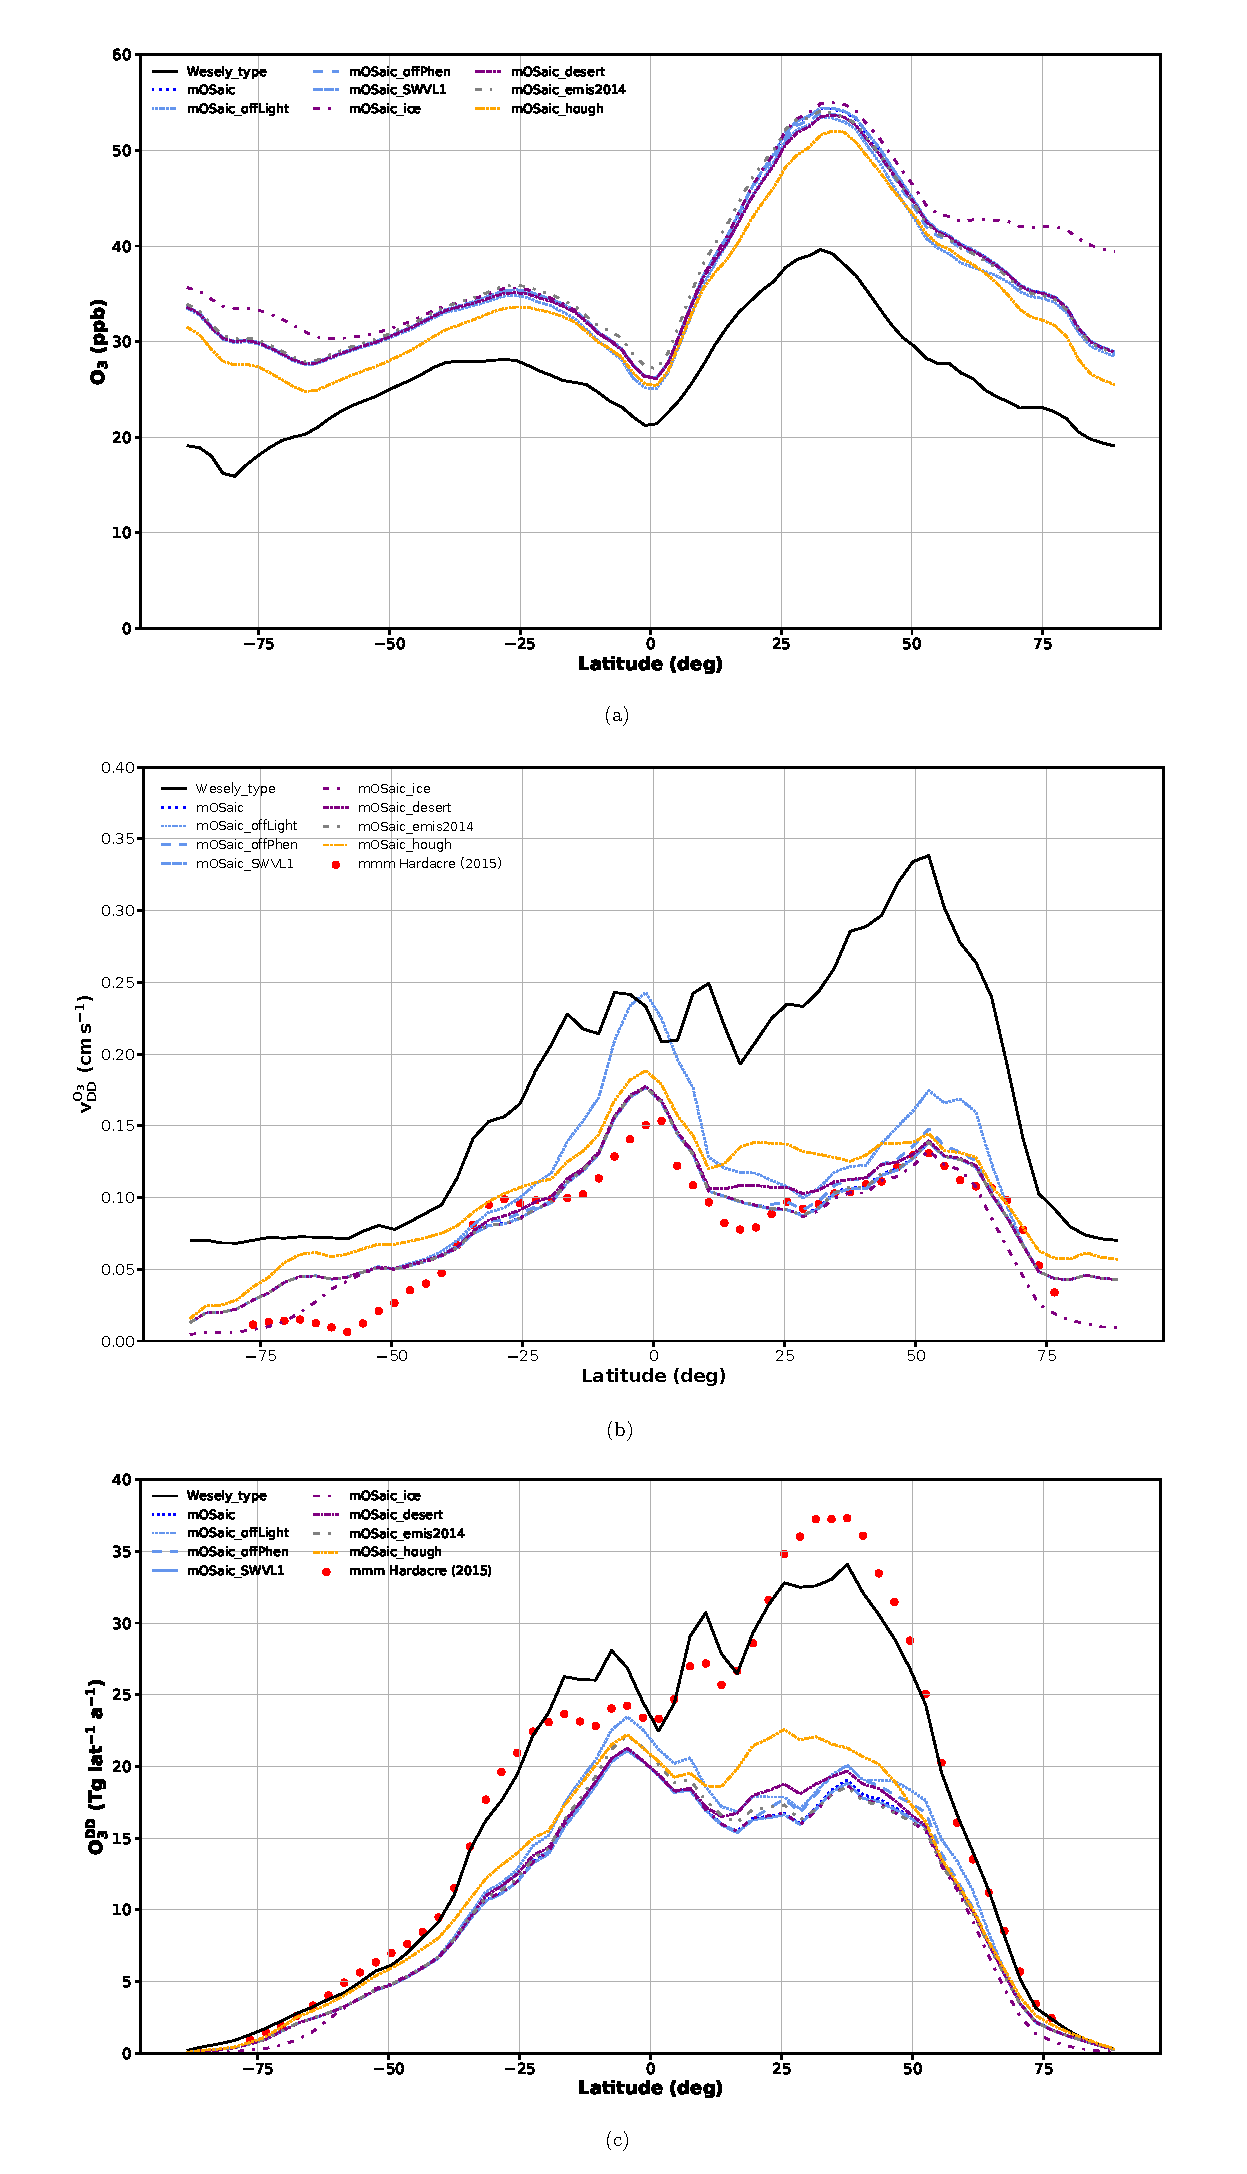
\includegraphics[width=8.3cm]{fig05}
  \caption{Comparison of the manifold of Oslo~CTM3 integrations with respect to (a) Ozone concentrations in the lowermost model level, (b) Annual average ozone dry deposition velocity, (c) Total annual ozone dry deposition. The different colors indicate sets of simulation with similar baselines. The multi-model mean from the evaluation of TF~HTAP models by \citet{ACP:Hardacre2015} is shown as a reference (where available).}
  \label{fig:mmm_drydep}
\end{figure}
%
In Appendix Fig.~\ref{fig:mmm_drydep_season}a, the average zonal ozone dry deposition is shown separated by month. Where available, we have added the multi-model-mean given by \citet{ACP:Hardacre2015} as a reference. As for the global annual comparisons above, the mOSaic scheme matches the multi-model-mean values remarkably well with respect to dry deposition velocities, while it strongly underestimates the total dry deposition. Qualitatively, there are two major phases apparent: NH and SH greening season. Spring and summer in the NH is reflected in a pronounced peak of $v_\text{DD}^\chem{O_3}$ in the northern mid latitudes, while it is absent in winter (SH summer). Spring and summer in the SH are marked by a southward shift of the tropical peak dry deposition velocity and a slight increase of $v_\text{DD}^\chem{O_3}$ in the region $(20-40)\,\unit{^\circ S}$. In the Wesely scheme, NH mid latitude peak velocities appear in June compared to July in the mOSaic scheme, indicating that the seasonal cycles differ. The corresponding total monthly ozone dry deposition is shown in Appendix Fig.~\ref{fig:mmm_drydep_season}b. In general, the seasonal patterns are quite similar in the Wesely scheme and the mOSaic scheme, displaying a strong symmetry around $10\,\unit{^\circ N}$ in January/February and November/December, respectively. What differs most is the molding and intensity of the NH peak dry deposition. Both schemes reach the maximum in June/July but the peak is much more differentiated in March already in the Wesely scheme. Similarly, the SH tropical peak dry deposition is reached in August/September but sustained longer, into October, in the Wesely scheme. Since we have not conducted any simulation with a meteorological year other than 2005, we cannot elaborate on whether this is a special feature of our chosen year or not.
%
%%%%%%%%%%%%%%%%%%%%%%%%%%%%%%%%%%%%%%%%
\subsubsection{Average seasonal cycles}
\label{subsubsec:seasons}
%
To further disentangle the contributions of different regions to the global ozone budget, we will look at different projections of seasonal cycles.

In Fig.~\ref{fig:mmm_drydep_hem}, the total annual ozone dry deposition separated into mid and high latitudes in the northern hemisphere ($30\,\unit{^\circ}-90\,\unit{^\circ N}$), the tropics and subtropics ($30\,\unit{^\circ S}-30\,\unit{^\circ N}$), and the mid and high latitudes in the southern hemisphere ($30\,\unit{^\circ}-90\,\unit{^\circ S}$) is shown. We have added the multi-model-mean by \citet{ACP:Hardacre2015} as a reference. While the total ozone dry deposition of \emph{Wesely\_type} agrees well with the multi-model-mean in any zonal band, the mOSaic scheme displays a much smaller total ozone dry deposition. This deviation appears to be almost the same for each zonal band ($6-7\,\unit{\%}$).

As expected, the NH mid and high latitudes display a strongly pronounced seasonal cycle, while it is less pronounced in the tropics (due to the lack of seasons) and in the SH (due to the small percentage of vegetated surface). The highest ozone dry deposition is found in the tropics and amounts on average to the  peak level of dry deposition in the NH for the multi-model-mean \citep{ACP:Hardacre2015} and mOSaic scheme. In the Wesely scheme, the average tropical ozone dry deposition diverges by $5\,\unit{Tg}$ in comparison to its corresponding NH maximum. Compared to the multi-model-mean, the seasonal cycle in the Oslo~CTM3 NH appears to be shifted towards later in the year. The seasonal cycle in the tropics and subtropics only differs by magnitude otherwise the shapes are identical for the mOSaic scheme, the Wesely scheme, and the multi-model-mean. The total amount of dry deposition of ozone differs strongly between the different model experiments, with \emph{mOSaic\_SWVL1} and \emph{mOSaic\_hough} displaying the lowest and highest amount, respectively. This indicates that surface ozone is much more sensitive to the choice of parameters ($\mathcal{O}(5\,\unit{ppb})$ for \emph{mOSaic\_hough} in the tropics) than to slight changes in precursor emissions ($\mathcal{O}(1\,\unit{ppb})$ for \emph{mOSaic\_emis2014} in the tropics).

As suggested by \citet{ACP:Hardacre2015}, we also look at ozone dry deposition velocities with respect to surface types separately. Since dry deposition velocities are not directly available for \emph{Wesely\_type}, we use Eq.~(\ref{eq:retro_vdd}) to estimate these. Based on a CLM~2 average dynamic land surface map, we generate masks for 9 different surface types (Fig.~\ref{fig:pft_landsurface}a) and use these to select gridboxes with a high percentage of these surface types, ranging from a meager $70\,\unit{\%}$ for cropland in the NH mid latitudes to $100\,\unit{\%}$ for desert, ocean, snow and ice, and tropical forest. Thus, it is not possible to exclusively select gridboxes with $100\,\unit{\%}$ cover for each surface type. Since we have not performed a full unfolding on the data, the results should be treated with slight caution (e.g. over cropland). In the case of the mOSaic scheme, we have pre-selected the dry deposition velocities in accordance to the land surface type.
%
\begin{figure*}[t]
  \includegraphics[width=12cm]{fig06}
  \caption{Seasonal cycle of total annual amount of ozone removed from the atmosphere through dry deposition separated into northern hemisphere (NH), tropics (TR), and southern hemisphere (SH). The multi-model mean from the evaluation of HTAP models by \citet{ACP:Hardacre2015} is shown as a reference.}
  \label{fig:mmm_drydep_hem}
\end{figure*}
%

In Fig.~\ref{fig:mmm_drydep_season_pft}, the seasonal cycles of dry deposition velocities are shown for the nine surface categories. The patterns and absolute numbers differ substantially between the Wesely scheme and the mOSaic scheme and the multi-model-mean. The divergence of the average dry deposition velocities between \emph{Wesely\_type} and \emph{mOSaic} in desert regions ($\Delta \overline{v}_\text{desert}^\chem{O_3} = 0.20\,\unit{cm\,s^{-1}}$) as well as grassland ($\Delta \overline{v}_\text{grassland}^\chem{O_3} = 0.65\,\unit{cm\,s^{-1}}$) is quite remarkable. The difference of \emph{mOSaic} and \emph{Wesely\_type} to the multi-model-mean in tropical forest regions is $\Delta_\text{mOSaic} \overline{v}_\text{tropical forest}^\chem{O_3} = 0.61\,\unit{cm\,s^{-1}}$ and $\Delta_\text{Wesely\_type} \overline{v}_\text{tropical forest}^\chem{O_3} = 0.49\,\unit{cm\,s^{-1}}$, respectively. The multi-model-mean displays a rather pronounced seasonal cycle in desert regions ($0.10\,\unit{cm\,s^{-1}} \leq v^\chem{O_3}_\text{desert}\leq 0.15\,\unit{cm\,s^{-1}}$), which cannot be reproduced with the mOSaic scheme. The dry deposition velocities over desert regions are consistent with the average values from the prescribed ozone surface resistances, which means that in the mOSaic scheme they are $1$ order of magnitude lower than in the Wesely scheme. In the mOSaic scheme, dry deposition to deserts is dominated by contribution from $R_b$. From a limited number of ozone flux measurements in the Sahara desert, \citet{AE:Gusten1995} deduced $v^\chem{O_3}_\text{desert, day} = 0.1\,\unit{cm\,s^{-1}}$, $v^\chem{O_3}_\text{desert, night} = 0.04\,\unit{cm\,s^{-1}}$, and $\overline{v}^\chem{O_3}_\text{desert} = 0.065\,\unit{cm\,s^{-1}}$. This implies, that ozone dry deposition over desert regions is highly overestimated in the Wesely scheme as well as in TF~HTAP models, while it may be underestimated in the mOSaic scheme. Similarly, the dry deposition velocities over water differ. From measurements during ship-campaigns a mean value of $\overline{v}^\chem{O_3}_\text{water} = 0.019\,\unit{cm\,s^{-1}}$ over the ocean has been deduced \citep{JGR:Helmig2012}. In a model study of different mechanisms of dry deposition to ocean waters by means of prescribed $\overline{v}_\text{water}^\chem{O_3}$ and one- and two-layer gas exchange modeling, \citet{ACP:Luhar2017} found $\overline{v}_\text{water}^\chem{O_3}$ ranging between $0.018\,\unit{cm\,s^{-1}}$ (two-layer scheme) and $0.039\,\unit{cm\,s^{-1}}$ (prescribed). With $\overline{v}^\chem{O_3}_\text{water} = (0.046\pm0.002)\,\unit{cm\,s^{-1}}$, the mOSaic scheme (Section~\ref{subsubsec:Rb}) yields probably a too strong dry deposition to ocean, but is in line with the multi-model-mean. This implies that ozone concentrations might even become larger and dry deposition even lower in the model if a more advanced dry deposition scheme to the ocean would be implemented. With respect to vegetation, we might be able to improve the model performance further by allowing more PFTs and phenologies, especially in regions covered by tropical forest \citep{GCB:Anav2017} or in boreal regions. 
%
\begin{figure*}[t]
  \includegraphics[width=12cm]{fig07}
  \caption{Average seasonal cycles of ozone dry deposition velocities separated by land use type. Results from \citep{ACP:Hardacre2015} are shown as a reference. We refrain from showing the full extent of \emph{EMEP\_offLight} here, since it is an extreme scenario and has been discussed already.}
  \label{fig:mmm_drydep_season_pft}
\end{figure*}
%

Finally, we take a look at the different global as well as hemispheric dry deposition sinks for ozone (Table~\ref{tab:ozone_sinks}). Despite its vastness, the ocean amounts only to $35\,\unit{\%}$ of the global ozone sink due to dry deposition in the Oslo~CTM3 with operative mOSaic scheme (\emph{mOSaic}), while permanently ice and snow covered regions account for $1.2\,\unit{\%}$. The remainder is deposited to land surfaces of which deserts might be the most neglected in process-modeling. The total annual dry deposition in the mOSaic scheme is one-third below the multi-model-mean result by \citet{ACP:Hardacre2015}. But also the results of \citet{ACP:Luhar2017, ACP:Luhar2018} yield a $(19-27)\,\unit{\%}$ lower ozone dry deposition than the models participating in the model intercomparison, with deposition to ocean ranging between $(12-21)\,\unit{\%}$ of the total annual ozone dry deposition. In particular, \citet{ACP:Luhar2018} found that current model estimates of ozone dry deposition to the ocean may be three times too high compared to their analysis. This implies that the ozone dry deposition to the ocean in the Oslo~CTM3 is too high as well.
%
\begin{table*}[t]
  \caption{Total ozone dry deposition for the respective model experiment in \unit{Tg\,a^{-1}}. The global ozone dry deposition has been weighted by ocean, ice and, land fraction in each gridbox, respectively. \emph{Ice} herein refers to regions at high latitudes that are permanently covered by ice and snow.}
  \begin{tabular}{lccccccccc|cccr}
    \tophline
    \multirow{3}{*}{Experiment} & \multicolumn{3}{c}{Ocean} & \multicolumn{3}{c}{Ice} & \multicolumn{3}{c}{Land} & \multicolumn{3}{c}{Total} & $\Delta^\dagger$\\
    & NH & SH & Global & NH & SH & Global & NH & SH & Global & NH & SH & Global\\
    & \multicolumn{3}{c}{(\unit{Tg\,a^{-1}})} & \multicolumn{3}{c}{(\unit{Tg\,a^{-1}})} & \multicolumn{3}{c}{(\unit{Tg\,a^{-1}})} & \multicolumn{3}{c}{(\unit{Tg\,a^{-1}})} & (\unit{\%})\\
    \middlehline
    Wesely\_type & 160.5 & 147.7 & 308.2 & 7.0 & 6.4 & 13.4 & 417.3 & 190.8 & 608.2 & 613.4 & 344.9 & 958.3 & 36.7\\
    mOSaic & 108.1 & 105.3 & 213.4 & 4.3 & 3.1 & 7.4 & 236.2 & 130.3 & 366.4 & 368.3 & 238.6 & 606.9 & 0.0\\
    mOSaic\_offLight & 110.5 & 106.3 & 216.8 & 4.3 & 3.0 & 7.4 & 263.1 & 145.3 & 408.4 & 399.9 & 254.7 & 654.6 & 7.3\\
    mOSaic\_offPhen & 108.3 & 105.3 & 213.6 & 4.3 & 3.1 & 7.4 & 246.9 & 132.2 & 379.1 & 379.5 & 240.5 & 620.0 & 2.1\\
    mOSaic\_SWVL1 & 108.1 & 105.2 & 213.3 & 4.3 & 3.1 & 7.4 & 234.6 & 128.8 & 363.4 & 366.6 & 237.1 & 603.7 & -0.5\\
    mOSaic\_ice & 105.6 & 103.0 & 208.6 & 2.6 & 1.0 & 3.6 & 232.7 & 130.2 & 362.9 & 358.3 & 234.2 & 592.6 & -2.4\\
    mOSaic\_desert & 109.1 & 105.5 & 214.6 & 4.3 & 3.1 & 7.4 & 250.4 & 132.6 & 383.0 & 383.4 & 241.2 & 624.6 & 2.8\\
    mOSaic\_emis2014 & 108.9 & 107.0 & 215.9 & 4.3 & 3.1 & 7.3 & 238.3 & 133.8 & 372.1 & 370.8 & 243.9 & 614.7 & 1.3\\
    mOSaic\_hough & 133.3 & 131.1 & 264.4 & 4.9 & 3.6 & 8.4 & 265.8 & 132.0 & 397.8 & 423.6 & 266.7 & 690.3 & 12.1\\
    \bottomhline
  \end{tabular}
  \belowtable{$^\dagger$: Relative change of global annual total in comparison to \emph{mOSaic}.}% Table Footnotes
  \label{tab:ozone_sinks}
\end{table*}

Table~\ref{tab:trop_ozone_burden} displays the average tropospheric ozone burden for all model experiments. Consistently with the previous findings, the mOSaic scheme increases the tropospheric ozone burden by $35\,\unit{Tg}$. From various satellite ozone retrieval products, \citet[][Tab.~5]{ESA:Gaudel2018} deduce a lower limit estimate for global tropospheric ozone burden for the years $2010-2014$ of $333-345\,\unit{Tg}$, but remark that this amount underestimates the actual tropospheric ozone burden, since it is only based on daytime retrievals. Nevertheless, the results of \emph{mOSaic} lie $17\,\unit{\%}$ above that estimate and also well above the typical modeling range of $302-378\,\unit{Tg}$ \citep{ACP:Young2013}. Despite the strong positive bias in ozone concentrations and accordingly low-bias in total dry deposition, the difference between \emph{mOSaic} and \emph{mOSaic\_emis2014} ($6\,\unit{Tg}$), lies well within the range given by satellites for the years 2005 and 2014 \citep[][Fig.~26]{ESA:Gaudel2018}. This indicates that the Oslo~CTM3 responds well to given changes in global emissions.
%
\begin{table*}[h]
  \caption{Annual mean tropospheric ozone burden for all experiments and $1 \sigma$ standard deviation.}
  \centering
  \begin{tabular}{lrcl}
    \tophline
    Experiment & \multicolumn{3}{c}{Trop. \chem{O_3}}\\
    &  \multicolumn{3}{c}{(Tg)}\\
    \middlehline
    Wesely\_type & 364 & $\pm$ & 23 \\
    mOSaic & 399 & $\pm$ & 31 \\
    mOSaic\_offLight & 395 & $\pm$ & 30 \\
    mOSaic\_offPhen & 398 & $\pm$ & 31 \\
    mOSaic\_SWVL1 & 399 & $\pm$ & 31 \\
    mOSaic\_ice & 401 & $\pm$ & 31 \\
    mOSaic\_desert & 398 & $\pm$ & 31 \\
    mOSaic\_emis2014 & 405 & $\pm$ & 32 \\
    mOSaic\_hough & 393 & $\pm$ & 30 \\
    \bottomhline
  \end{tabular}
  \label{tab:trop_ozone_burden}
\end{table*}

%%%%%%%%%%%%%%%%%%%%%%%%%%%%
\subsection{Comparison with MACC-reanalysis}
\label{subsec:macc}
In this section, we conclude the comparison of our results with respect to global ozone by looking at ECWMF's MACC-reanalysis \citep[][data obtained from \href{https://apps.ecmwf.int/datasets/data/macc-reanalysis/levtype=ml/}{ECWMF's data center}]{MACC-II}.
In Fig,~\ref{fig:macc_o3conc}, we compare \emph{mOSaic} ozone concentrations in the lowermost model level with surface concentrations deduced from the MACC-reanalysis for the year 2005. The MACC-reanalysis displays low ozone concentrations above all land masses except for the Greenland ice sheet. The lowest values are found in the deep tropics (e.g. northern South America and central Africa), while the highest values occur within $(25-60)\,\unit{^\circ N}$ over the oceans. These low values over the oceans are relatively well reproduced by \emph{mOSaic} ($\pm 20\,\unit{\%}$). Over, e.g., South America, central and southern Africa, the Arabian peninsula, and the north-western Indian subcontinent, the ozone concentrations are elevated by up to $200\,\unit{\%}$.
Regarding the global average surface ozone concentration, \emph{Wesely\_type} (Supplement S.8) is more consistent with the MACC-reanalysis than \emph{mOSaic}, but shows the same tendency of enhanced ozone over the continents as the latter.
This enhancement is apparent mostly in the deep tropics and over the north-western Indian subcontinent which coincides with regions of high intensity in incoming UV radiation. This may indicated an imbalance in the photo-chemical production and loss of \chem{O_3} in the Oslo~CTM3.

\begin{figure}[t]
  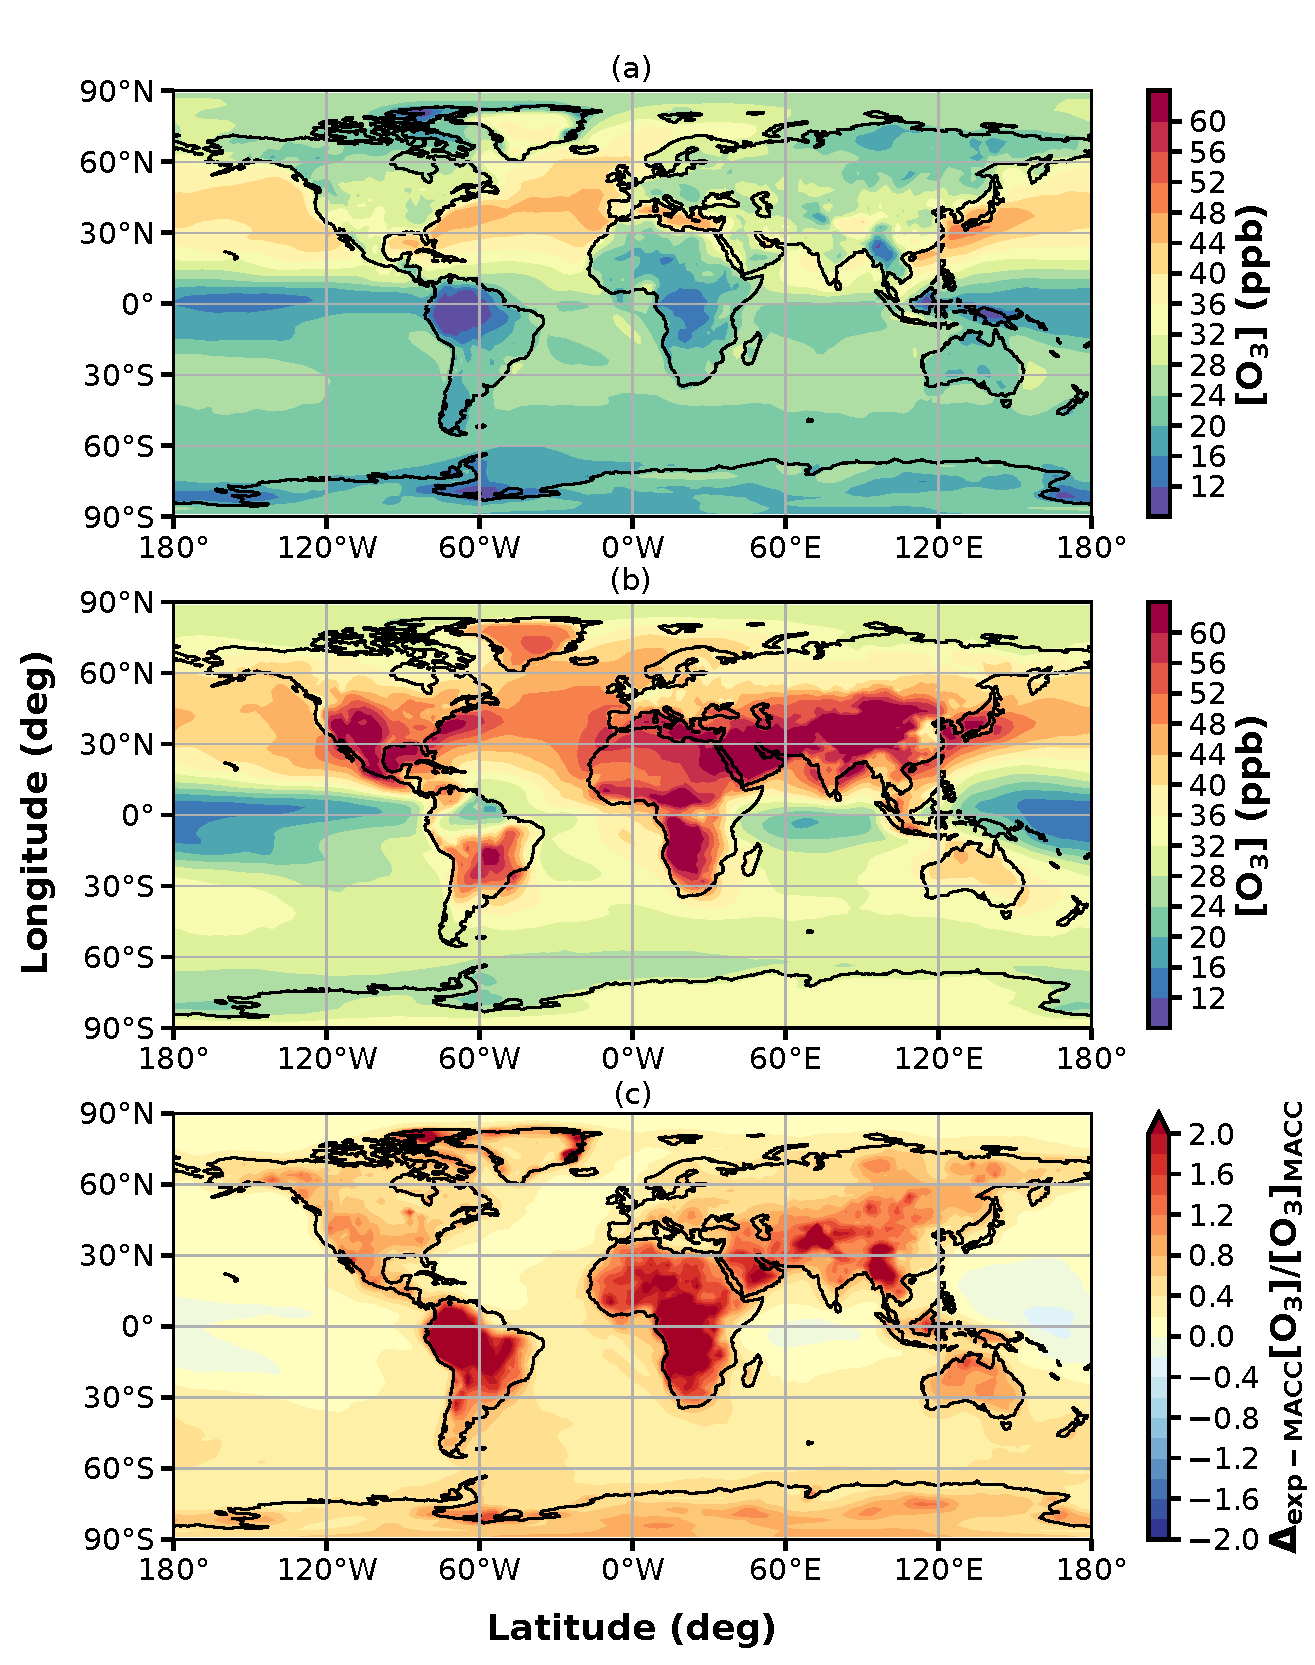
\includegraphics[width=8.3cm]{fig08}
  \caption{Mean ozone concentrations for the year 2005. (a) MACC-reanalysis (surface); (b) Oslo~CTM3 \emph{mOSaic} (lowermost model level); (c) Relative difference.}
  \label{fig:macc_o3conc}
\end{figure}

%%%%%%%%%%%%%%%%%%%%%%%%%%%%
\subsection{Comparison with ground-based observations}
\label{subsec:obs}
In this section, we compare our model results to observations at a selected number of sites which provide ozone flux measurements. For all comparisons, we use the original resolution of the Oslo~CTM3 ($2.25^\circ\times 2.25^\circ$) instead of the re-gridded resolution ($3^\circ\times 3^\circ$).

In Fig.~\ref{fig:mmm_drydep_stations}a, seasonal cycles of average ozone dry deposition fluxes for the six selected observation sites are shown. We have computed a model average for all sensitivity studies at the closest grid point and show the $1\,\sigma$ uncertainty band. The shaded area around the multi-model-mean indicates the broad range of model results but is not an actual uncertainty band since such is not given in \citet{ACP:Hardacre2015}. At $4$ of the $6$ sites, the mOSaic scheme performs better than the Wesely scheme and similar to or better than the multi-model-mean. We use a $\chi^2$-test
\begin{equation}
  \chi^2 = \sum_{i=1}^{12}\frac{\left(\overline{\chem{O_3}}_{\text{DD,\,}i}^\text{sim}-\overline{\chem{O_3}}_{\text{DD,\,}i}^\text{obs}\right)^2}{\sigma_i^2},
\end{equation}
with an estimated standard deviation of observation $\sigma_i=1\,\unit{mmol\,m^{-2}\,s^{-1}}$ and divide it by the number of degrees of freedom (NDF) to assess this subjective analysis in a more objective way. The closer to $1$ this test scores, the better does the simulation represent the observation. A score between $0$ and $1$ indicates that the estimated $\sigma$ is too small. The results of the $\chi^2$-test are shown together with the divergences in Fig.~\ref{fig:mmm_drydep_stations}b. The $\chi^2$-test reveals also that in $4$ of the $6$ cases the mOSaic scheme improves the performance of the Oslo~CTM3 with respect to observed ozone dry deposition fluxes, although a satisfying result is only achieved for two sites (Castel Porziano, Blodgett Forest).
With only one full year of simulation, the model uncertainty regarding the seasonal cycle at observational sites cannot be properly quantified. Furthermore, the observational averages comprise at most $9$ years worth of data. Statistically, these data may still be subject to interannual variability. Among other aspects, the horizontal as well as vertical resolution play an important role in the model performance. Although, we do not explicitly assess the impacts of differing resolutions in our model, we can assume that both high and low biases exist due to dilution of sources and sinks in coarse resolution models \citep{AE:Schaap2015}. Good matches between observation and model are only to be expected if the station's location is representative for an area similar to the respective model gridbox and not substantially affected by differences in modeled and actual topography (e.g., major wind directions).

%
\begin{figure}[t]
  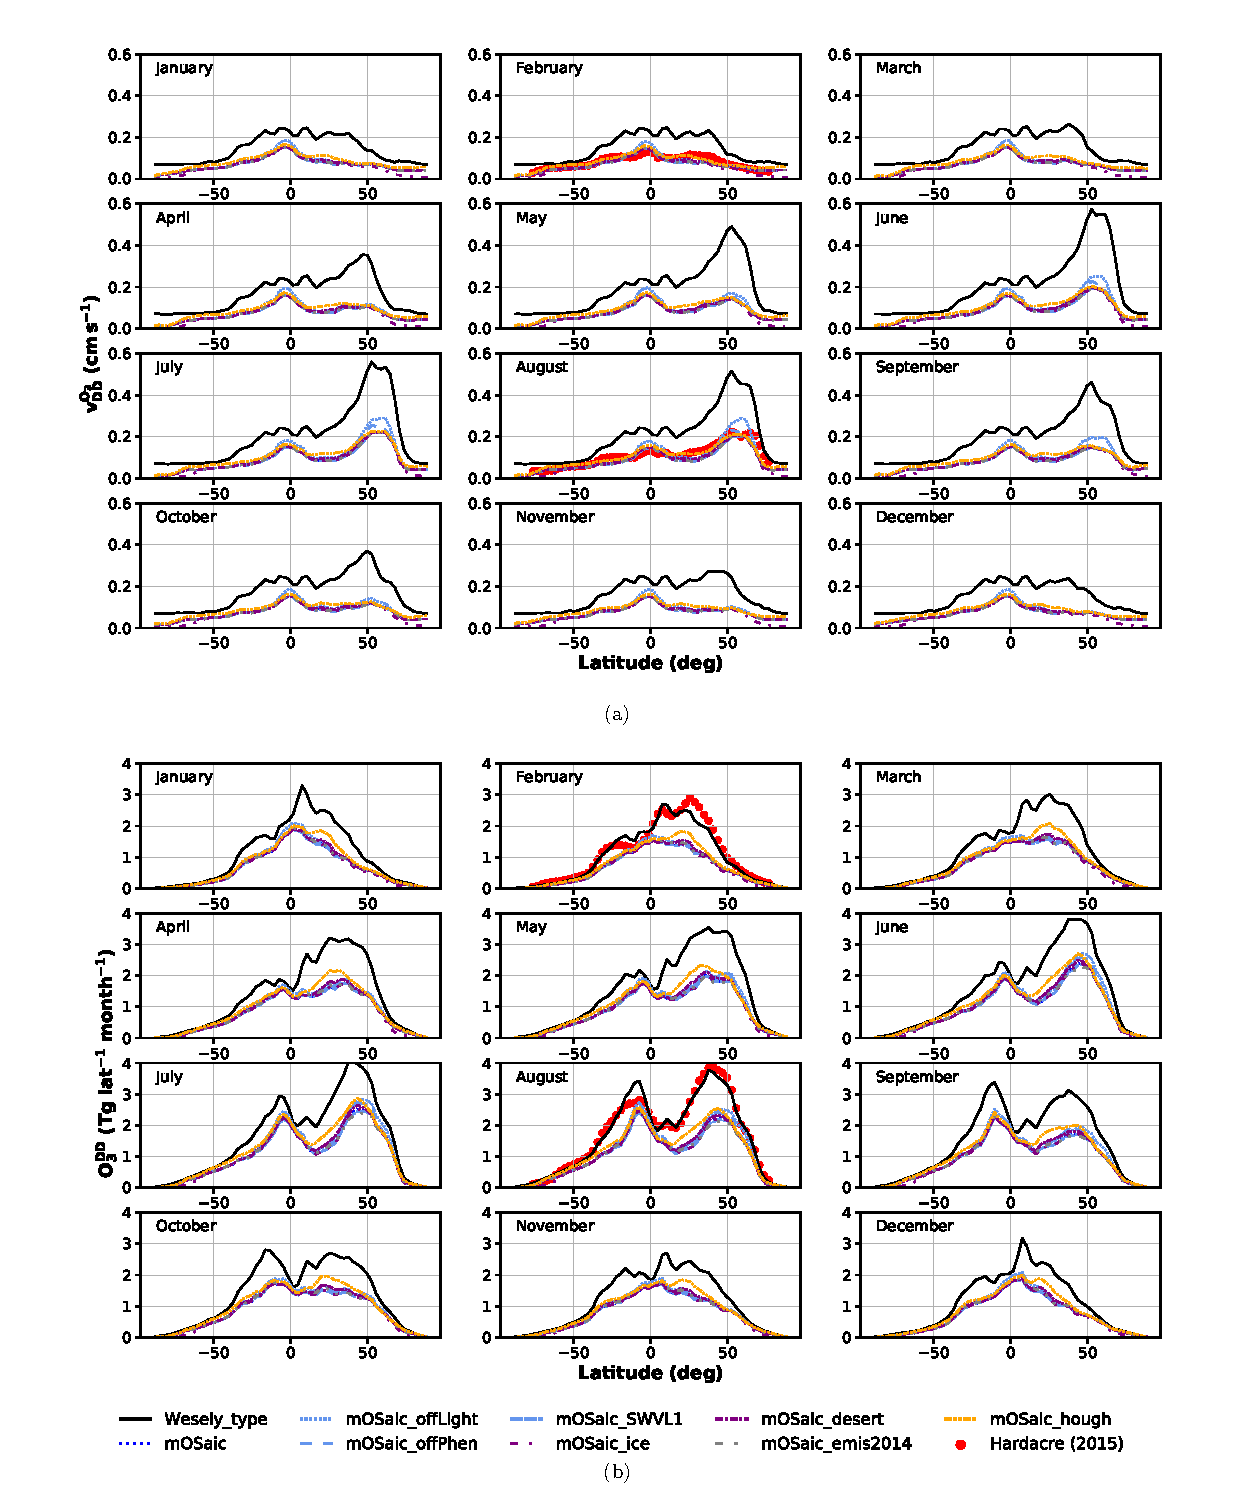
\includegraphics[width=8.3cm]{fig09}
  \caption{Ozone dry deposition fluxes at different observation sites. (a) Comparison between Wesely scheme and average result from all sensitivity studies with observational averages taken from \citet{ACP:Hardacre2015}. The model uncertainty of the Oslo~CTM3 is given as $1\,\sigma$ error band. The shaded area around the multi-model-mean indicates the broad range of different model results but is not an actual error band. (b) Model divergence from observation and $\chi^2$-test results.}
  \label{fig:mmm_drydep_stations}
\end{figure}

%%%%%%%%%%%%%%%%%%%%%%%%%%%%
\conclusions[Summary and conclusions]  %% \conclusions[modified heading if necessary]
\label{sec:conc}
We have presented an update of the dry deposition scheme in the Oslo~CTM3 from purely prescribed dry deposition velocities \citep{AE:Wesely1989,JGR:Hough1991} to a more process-oriented parameterization taking the state of the atmosphere and vegetation into account. Based on the description of dry deposition in \citet{WASP:Simpson2003,ACP:Simpson2012}, we have implemented a mosaic approach to compute contributions to dry deposition by individual sub-grid land surface types. Aerodynamic, quasi-laminar, and surface resistance (with the latter divided into stomatal and non-stomatal contributions) are calculated for each land surface category separately. Based on these, a land fraction-weighted mean is deduced. In addition, the various dry deposition velocities are now directly available from model output for diagnostics and further studies.

The new dry deposition scheme named \emph{mOSaic} improves the modeled dry deposition velocities which are now compatible with observation and model studies \citep[e.g.,][]{ACP:Hardacre2015,ACP:Luhar2018}. Dry deposition velocities are reduced by $6-60\,\unit{\%}$. At the same time, the annual amount of ozone dry deposition decreases by more than $100\,\unit{\%}$ over all major desert areas and increases over tropical forest. Compared to results from a multi-model evaluation \citep{ACP:Hardacre2015}, the total annual ozone dry deposition in the Oslo~CTM3 is $(38\substack{+~\,1 \\ -10})\,\unit{\%}$ below average. However, there seems to be a tendency that newer TF~HTAP models show a lower total annual dry deposition of ozone than older models, indicating that newer developments lead to decreasing ozone dry deposition and increasing tropospheric ozone burden \citep[e.g.,][]{ACP:Luhar2017,ACP:Luhar2018,AE:Hu2017}.

We found the response of the Oslo~CTM3 to the changes in dry deposition velocities from the old and the mOSaic scheme to be consistent. A decrease in $v_\text{DD}^\chem{O_3}$ leads to a decrease in total ozone dry deposition and an increase in ozone concentration $[\chem{O_3}]$. As the new scheme is quantitatively more similar to the multi-model-mean \citep{ACP:Hardacre2015} with respect to dry deposition velocities, while the old scheme agrees better in terms of total dry deposition, there is an apparent discrepancy. By means of tropospheric ozone burden \citep{ESA:Gaudel2018} and surface ozone concentrations deduced from the MACC-reanalysis \citep{MACC-II}, the Oslo~CTM3 with the operational mOSaic scheme shows a pronounced high-bias of tropospheric ozone. While the average bias is small or even reversed when using the old scheme, both display elevated ozone in comparison with the MACC-reanalysis in continental regions with high average incoming UV radiation (e.g., northern South America, central and southern Africa, the Himalayas).
The reason behind this bias has not yet been resolved and may hint to, e.g., issues in photo-chemistry ($[\chem{OH}]$ related ozone production and loss) or previously introduced optimization of ozone removal with respect to the old, less physical dry deposition velocities.

Most of the qualitative change in ozone dry deposition in the Oslo~CTM3 ($-2-12\,\unit{\%}$) can be attributed to changes in dry deposition over the ocean and deserts. This is mainly due to updates of the respective, prescribed ozone surface resistances $R^\chem{O_3}$. In the case of desert and grasslands the difference between the old and new prescribed value is an order of magnitude. Over the ocean, the absolute change in dry deposition is small, but it is accumulated over a large area which is especially amplified in the southern hemisphere. Small adjustments to the lower limits in our quasi-laminar layer resistance formulation may help improve the Oslo~CTM3 performance in this regard. With respect to available measurements of dry deposition velocities of ozone over desert \citep{AE:Gusten1995} and ocean \citep{JGR:Helmig2012}, the new Oslo~CTM3 dry deposition scheme slightly underestimates ozone dry deposition velocities over the former and overestimate them over the latter. Regarding the vastness of the ocean and the ongoing desertification, it may be worthwhile to revise the dry deposition scheme for these regimes and add more process-oriented formulations, e.g., 2-layer gas exchange with ocean waters \citep{ACP:Luhar2017, ACP:Luhar2018}, wave breaking and spray \citep{ACP:Pozzer2006}.

Although dry deposition to ice and snow amounts to only $1\,\unit{\%}$ of the total global annual ozone dry deposition in \emph{mOSaic}, a decrease in prescribed dry deposition velocity in accordance to combined measurements and model studies \citep{ACP:Helmig2007} causes almost a doubling in the surface ozone concentrations in the high Arctic and affects surface ozone concentrations down to latitudes at $50\,\unit{^\circ}$ in both hemispheres. Comparing with results from the multi-model evaluation \citep{ACP:Hardacre2015}, we conclude that it is important to use this updated ozone dry deposition velocity to counter an Arctic surface ozone low-bias in models, however, this currently leads to an overcompensation (high-bias) in the Oslo~CTM3.

We have studied the parameter space of the stomatal conductance parameterization and found that surface ozone in the tropics and the northern hemisphere is most sensitive to changes therein. In the most extreme test case, the increase in global total dry deposition amounts to $7.3\,\unit{\%}$, while the more realistic test cases, e.g. using differing years of emission amount to changes of the order of $\pm 2\,\unit{\%}$. This may indicate that future changes in vegetation cover and solar radiation at the surface due to changes in stratospheric ozone, cloud cover, or aerosols could also strongly influence the surface ozone burden in the tropics. Total column ozone in the tropics is predicted to decrease due to changes in the atmospheric circulation \citep[e.g.,][]{WMO2014}, while tropospheric and surface ozone increase. The combined effects of increasing emissions of ozone precursors and an increase in UV due to thinning of stratospheric ozone might permit more UV light at ground and thus increase the ozone production.

%In the northern hemisphere mid and high latitudes ($50\,\unit{^\circ}-75\,\unit{^\circ N}$), total surface ozone increases by $7.7\,\unit{\%}$ if the beginning and end of the vegetation period is estimated based on a $5\,\unit{^\circ C}$-days criteria instead of prescribed. This is very important for any study focusing on ozone in the boreal and subarctic regions.

An important factor in the global ozone budget are emissions of precursor substances. We cover this by using the same meteorology with different years of CEDS emissions. We chose the years 2005 and 2014 for our comparison. Ozone precursor emissions in 2014 are slightly lower in the NH while enhanced in the tropics and the SH. In 2014, surface ozone burden is higher in the southern hemisphere and in the tropics ($5\,\unit{\%}$) compared to 2005, while it is lower in the northern hemisphere ($2\,\unit{\%}$).

We also evaluated the model with respect to observed dry deposition fluxes at six sites in the northern hemisphere and found that the mOSaic scheme performs better than the old one, but is not able to reproduce the measurements at most sites quantitatively. This may be due to several reasons. The model resolution in both horizontal ($2.25^\circ\times 2.25^\circ$) and vertical (L60, $P_\text{max}=0.02\,\unit{hPa}$) does not capture all details in transport, thus affecting the distribution and transport (e.g., long-range, convection, and stratosphere--troposphere exchange) of ozone and its precursors. Depending on the location of the observation site and its respective representativeness for a larger area, ozone dry deposition and ozone concentrations are expected to be over- or underestimated in the model. Because of non-linearities in ozone formation and destruction, ozone concentrations are sensitive to both, differences in local concentration of precursors and meteorological conditions \citep{JGR:Jin2013}. In addition, a comparison of very few years of measurement to only one specific year of simulation may reflect the year to year variability more than the actual model performance.

Future work on the Oslo~CTM3 should resolve the ozone high-bias which may involve revising the photolysis- and chemical reaction computation as well as reaction rates. For a better modeling of ozone abundances, ocean emissions of very short-lived ozone depleting substances (VSLS) \citep{JGR:Warwick2006, ACP:Ziska2013} which affect stratospheric ozone \citep{ACP:Hossaini2016, ACP:Falk2017} and a scheme covering Arctic spring-time ozone depletion \citep[e.g.,][]{ACP:Yang2010, ACP:Toyota2011, GMD:Falk2018}, could be worthwhile implementing. The general model performance could also be improved by allowing for more plant functional types and phenologies than currently used or implementing an actual photosynthesis-based modeling of plants. A more efficient parallelization of the code would enable computation at higher horizontal resolutions.

%% The following commands are for the statements about the availability of data sets and/or software code corresponding to the manuscript.
%% It is strongly recommended to make use of these sections in case data sets and/or software code have been part of your research the article is based on.

%\codeavailability{TEXT} %% use this section when having only software code available


%\dataavailability{TEXT} %% use this section when having only data sets available


\codedataavailability{The Oslo~CTM3 shall be publicly available on git-hub under a MIT license in the future. Until then, access can be made granted under request. Model results can be made available under request.} %% use this section when having data sets and software code available


%\sampleavailability{TEXT} %% use this section when having geoscientific samples available
%\videosupplement{TEXT} %% use this section when having video supplements available


%\clearpage

\appendix
\section{Figures}    %% Appendix A

\appendixfigures
\begin{figure}[!htbp]
  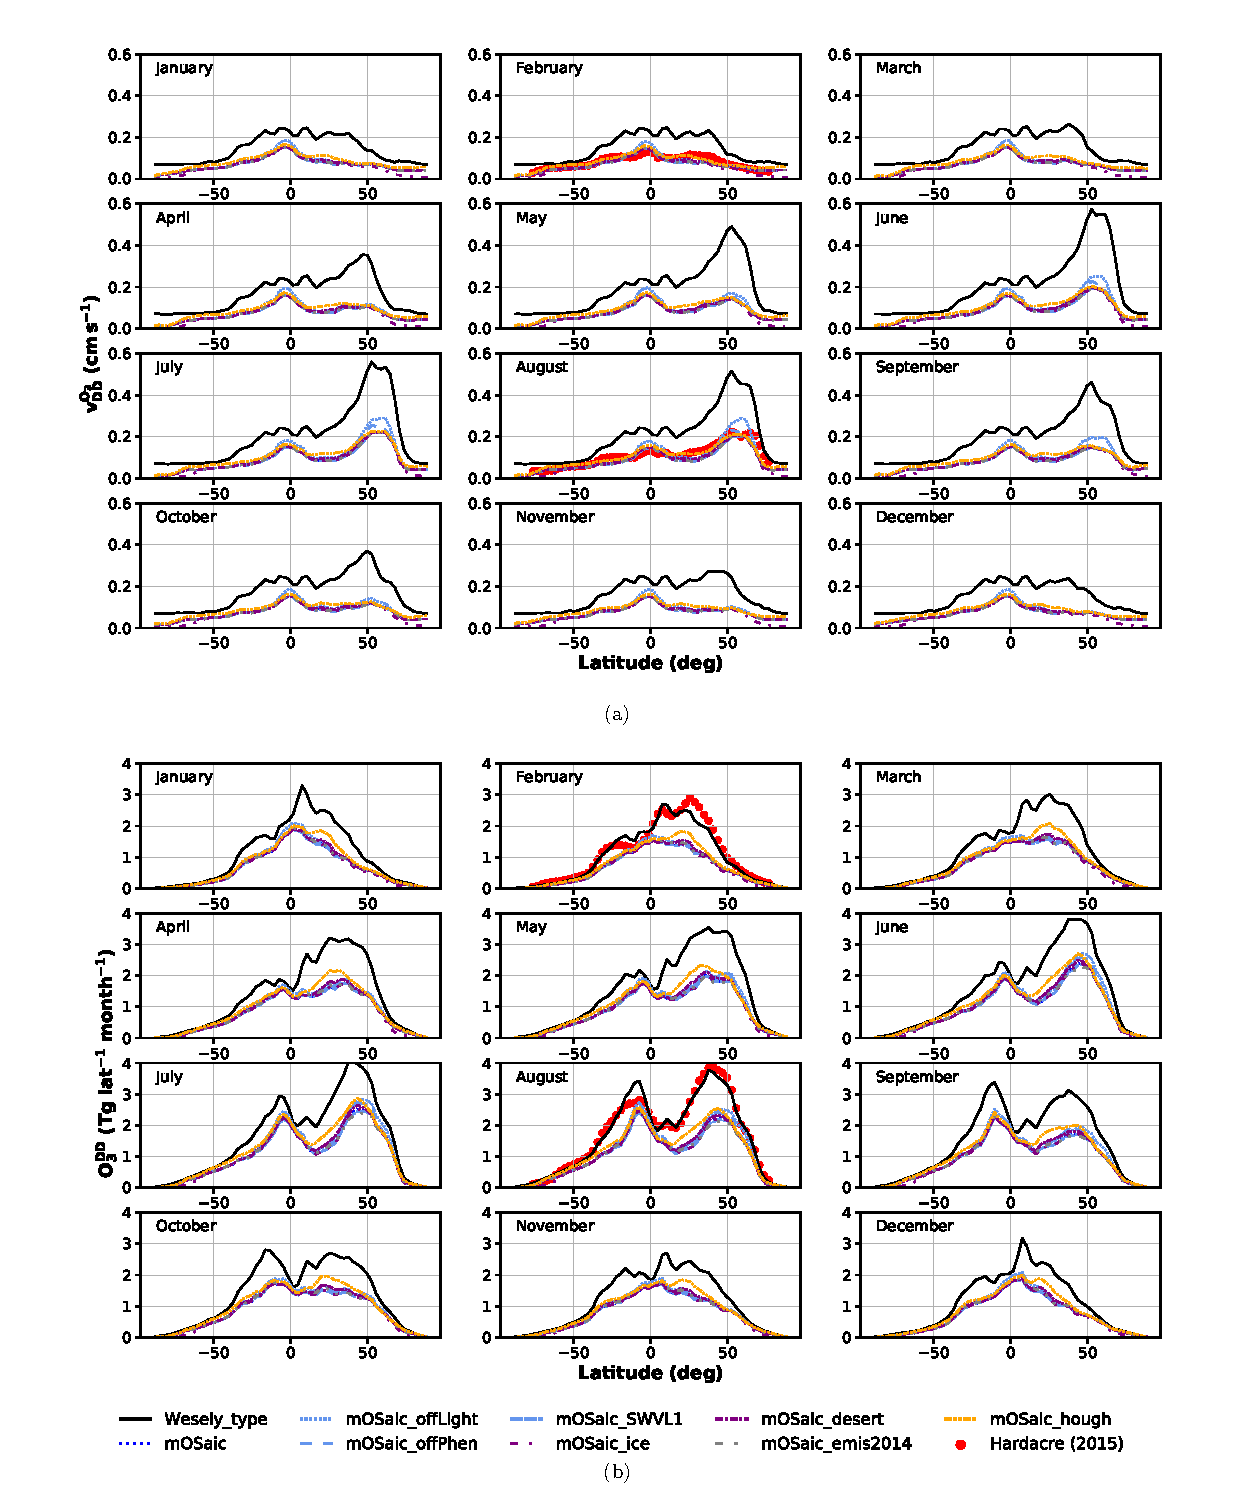
\includegraphics[width=0.8\textwidth]{fig10}
  \caption{Comparison of the manifold of Oslo~CTM3 integrations with respect to (a) Zonal average ozone dry deposition velocities; (b) Total annual amount of ozone removed from the atmosphere via dry deposition. The multi-model mean from the evaluation of TF~HTAP models by \citet{ACP:Hardacre2015} is shown as a reference (where available).}
  \label{fig:mmm_drydep_season}
\end{figure}

\appendixfigures
\begin{figure*}[!htbp]
  \centering
  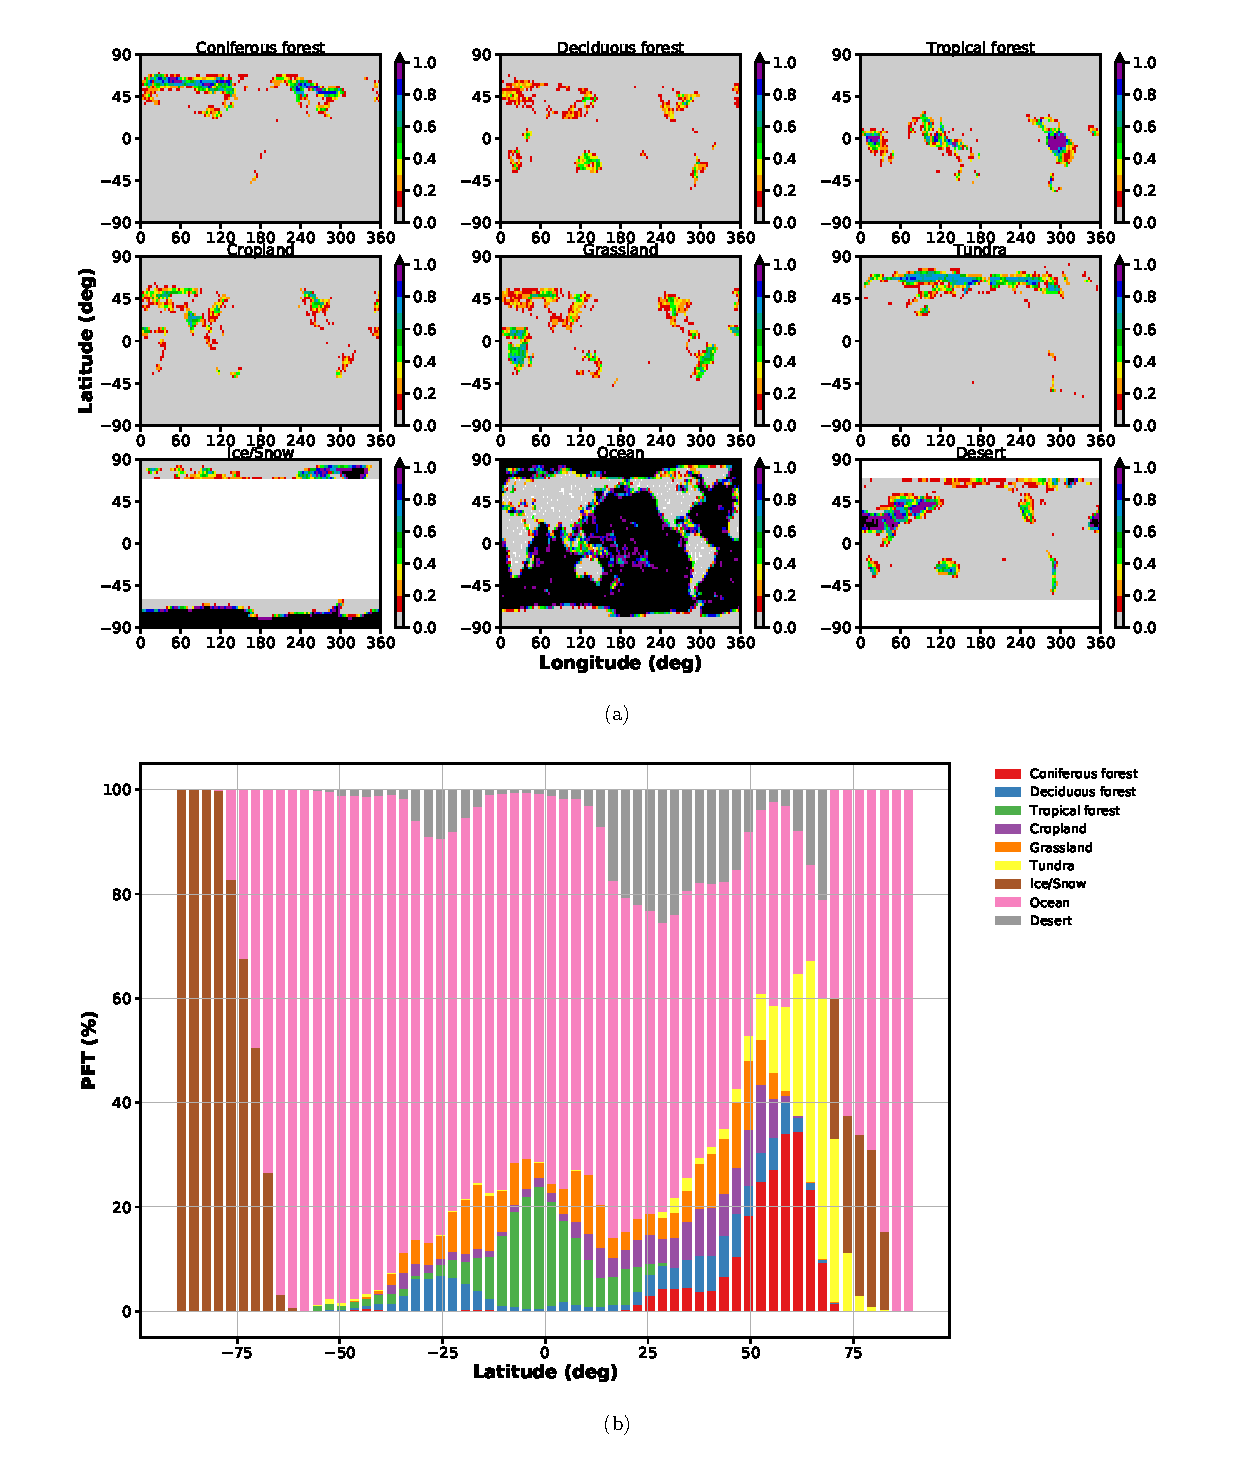
\includegraphics[width=0.8\textwidth]{fig11}
  \caption{Partitioning of land surface types. (a) CLM~2 dynamic land surface types in $(0.5\times0.5)\,\unit{^\circ}$ resolution; (b) Zonal distribution of land surface types.}
  \label{fig:pft_landsurface}
\end{figure*}

%\subsection{}     %% Appendix A1, A2, etc.


\noappendix       %% use this to mark the end of the appendix section

%% Regarding figures and tables in appendices, the following two options are possible depending on your general handling of figures and tables in the manuscript environment:

%% Option 1: If you sorted all figures and tables into the sections of the text, please also sort the appendix figures and appendix tables into the respective appendix sections.
%% They will be correctly named automatically.

%% Option 2: If you put all figures after the reference list, please insert appendix tables and figures after the normal tables and figures.
%% To rename them correctly to A1, A2, etc., please add the following commands in front of them:

%\appendixfigures  %% needs to be added in front of appendix figures

%\appendixtables   %% needs to be added in front of appendix tables

%% Please add \clearpage between each table and/or figure. Further guidelines on figures and tables can be found below.



\authorcontribution{Stefanie Falk has compiled the manuscript, finalized and revised the implementation of the stomatal conductance in the \emph{mOSaic} dry deposition scheme of the Oslo~CTM3, conducted the simulations, and analyzed and evaluated the results. Amund S{\o}vde Haslerud has implemented the \emph{mOSaic} dry deposition scheme and wrote the respective documentation. Both authors contributed to the writing and discussion of the paper.} %% this section is mandatory for the journals ACP and GMD. For all other journals it is strongly recommended to make use of this section

\competinginterests{The authors declare that they have no conflict of interest.} %% this section is mandatory even if you declare that no competing interests are present

%\disclaimer{TEXT} %% optional section

\begin{acknowledgements}
  This work was supported by the Norwegian Research Council (NRC) through the project The double punch: Ozone and climate stresses on vegetation (268073).\\
  The simulations were performed on resources provided by UNINETT Sigma2 -- the National Infrastructure for High Performance Computing and Data Storage in Norway (project nn2806k).\\
  The used Leaf Area Index (LAI) and roughness length ($z_0$) are available online from Oak Ridge National Laboratory Distributed Active Archive Center, Oak Ridge, Tennessee, U.S.A. (\doi{10.3334/ORNLDAAC/970}).\\
  Community Emission Data System (CEDS) historical emission inventory is provided by the Joint Global Research Institute project (\url{http://www.globalchange.umd.edu/ceds/}.)
  Randerson, J.T., G.R. van der Werf, L. Giglio, G.J. Collatz, and P.S. Kasibhatla. 2018. Global Fire Emissions Database, Version 4, (GFEDv4). ORNL DAAC, Oak Ridge, Tennessee, USA. https://doi.org/10.3334/ORNLDAAC/1293
  We would like to thank Prof. Frode Stordal (Section for Meteorology and Oceanography, University of Oslo) for discussions regarding early drafts of the manuscript, Anne Fouilloux (scientific programmer at the same institute) for technical support as well as Olimpia Bruno (Karlsruhe Institute of Technology) and Franziska Hellmuth (University of Oslo) for valuable input regarding the aerodynamic resistance formulation.
  We would also like to thank the Center for International Climate Research (CICERO) for their support of this work.
\end{acknowledgements}




%% REFERENCES

%% The reference list is compiled as follows:

%% Since the Copernicus LaTeX package includes the BibTeX style file copernicus.bst,
%% authors experienced with BibTeX only have to include the following two lines:
%%
\bibliographystyle{copernicus}
\bibliography{DryDep.bib}
%%
%% URLs and DOIs can be entered in your BibTeX file as:
%%
%% URL = {http://www.xyz.org/~jones/idx_g.htm}
%% DOI = {10.5194/xyz}


%% LITERATURE CITATIONS
%%
%% command                        & example result
%% \citet{jones90}|               & Jones et al. (1990)
%% \citep{jones90}|               & (Jones et al., 1990)
%% \citep{jones90,jones93}|       & (Jones et al., 1990, 1993)
%% \citep[p.~32]{jones90}|        & (Jones et al., 1990, p.~32)
%% \citep[e.g.,][]{jones90}|      & (e.g., Jones et al., 1990)
%% \citep[e.g.,][p.~32]{jones90}| & (e.g., Jones et al., 1990, p.~32)
%% \citeauthor{jones90}|          & Jones et al.
%% \citeyear{jones90}|            & 1990



%% FIGURES

%% When figures and tables are placed at the end of the MS (article in one-column style), please add \clearpage
%% between bibliography and first table and/or figure as well as between each table and/or figure.


%% ONE-COLUMN FIGURES

%%f
%\begin{figure}[t]
%\includegraphics[width=8.3cm]{FILE NAME}
%\caption{TEXT}
%\end{figure}
%
%%% TWO-COLUMN FIGURES
%
%%f
%\begin{figure*}[t]
%\includegraphics[width=12cm]{FILE NAME}
%\caption{TEXT}
%\end{figure*}
%
%
%%% TABLES
%%%
%%% The different columns must be seperated with a & command and should
%%% end with \\ to identify the column brake.
%
%%% ONE-COLUMN TABLE
%
%%t
%\begin{table}[t]
%\caption{TEXT}
%\begin{tabular}{column = lcr}
%\tophline
%
%\middlehline
%
%\bottomhline
%\end{tabular}
%\belowtable{} % Table Footnotes
%\end{table}
%
%%% TWO-COLUMN TABLE
%
%%t
%\begin{table*}[t]
%\caption{TEXT}
%\begin{tabular}{column = lcr}
%\tophline
%
%\middlehline
%
%\bottomhline
%\end{tabular}
%\belowtable{} % Table Footnotes
%\end{table*}
%
%%% LANDSCAPE TABLE
%
%%t
%\begin{sidewaystable*}[t]
%\caption{TEXT}
%\begin{tabular}{column = lcr}
%\tophline
%
%\middlehline
%
%\bottomhline
%\end{tabular}
%\belowtable{} % Table Footnotes
%\end{sidewaystable*}
%
%
%%% MATHEMATICAL EXPRESSIONS
%
%%% All papers typeset by Copernicus Publications follow the math typesetting regulations
%%% given by the IUPAC Green Book (IUPAC: Quantities, Units and Symbols in Physical Chemistry,
%%% 2nd Edn., Blackwell Science, available at: http://old.iupac.org/publications/books/gbook/green_book_2ed.pdf, 1993).
%%%
%%% Physical quantities/variables are typeset in italic font (t for time, T for Temperature)
%%% Indices which are not defined are typeset in italic font (x, y, z, a, b, c)
%%% Items/objects which are defined are typeset in roman font (Car A, Car B)
%%% Descriptions/specifications which are defined by itself are typeset in roman font (abs, rel, ref, tot, net, ice)
%%% Abbreviations from 2 letters are typeset in roman font (RH, LAI)
%%% Vectors are identified in bold italic font using \vec{x}
%%% Matrices are identified in bold roman font
%%% Multiplication signs are typeset using the LaTeX commands \times (for vector products, grids, and exponential notations) or \cdot
%%% The character * should not be applied as mutliplication sign
%
%
%%% EQUATIONS
%
%%% Single-row equation
%
%\begin{equation}
%
%\end{equation}
%
%%% Multiline equation
%
%\begin{align}
%& 3 + 5 = 8\\
%& 3 + 5 = 8\\
%& 3 + 5 = 8
%\end{align}
%
%
%%% MATRICES
%
%\begin{matrix}
%x & y & z\\
%x & y & z\\
%x & y & z\\
%\end{matrix}
%
%
%%% ALGORITHM
%
%\begin{algorithm}
%\caption{...}
%\label{a1}
%\begin{algorithmic}
%...
%\end{algorithmic}
%\end{algorithm}
%
%
%%% CHEMICAL FORMULAS AND REACTIONS
%
%%% For formulas embedded in the text, please use \chem{}
%
%%% The reaction environment creates labels including the letter R, i.e. (R1), (R2), etc.
%
%\begin{reaction}
%%% \rightarrow should be used for normal (one-way) chemical reactions
%%% \rightleftharpoons should be used for equilibria
%%% \leftrightarrow should be used for resonance structures
%\end{reaction}
%
%
%%% PHYSICAL UNITS
%%%
%%% Please use \unit{} and apply the exponential notation


\end{document}
